\documentclass[a4paper,10pt]{report}

\usepackage{packages/rapportutc}
%\usepackage{packages/include-packages}


%%%%%%%% Références %%%%%%%%
\usepackage{cleveref}
\usepackage{hyperref}
\usepackage[nottoc, notlof, notlot]{tocbibind} % bibliographie http://tex.stackexchange.com/questions/71129/bibliography-in-table-of-contents
\usepackage{natbib} % bibliographie

%%%%%%%% Code informatique %%%%%%%%
\usepackage{packages/Sweave} %package d'affichage des codes R
\usepackage{listings} % pour hightlight code

%%%%%%%% Formules mathématiques %%%%%%%%
\usepackage{amsmath, amsthm, amssymb, graphics, setspace} %packages de mathématiques
\usepackage{chemist} %formule chimique 

%%%%%%%% Mise en forme %%%%%%%%
% Mise en forme graphique
\usepackage{graphicx,wrapfig,lipsum} % pour afficher des figures à côté du texte
\usepackage[linewidth=1pt]{mdframed} % permet de générer et gérer des frames
\usepackage{rotating} % rotations on tables, captions, text, ...
% Mise en forme images et tableaux
\usepackage{float} % permet de spécifier l'option "H" aux captions afin de les positionner de manière fixe
\usepackage{subcaption} % permet d'afficher plusieurs images dans une caption
\usepackage{array} % meilleurs "table" et "tabular"
% Mise en forme texte
\usepackage{setspace} % permet de spécifier l'espacement interligne
\usepackage{ulem} % \sout{Texte à barrer} \xout{Texte à hachurer} \uwave{Texte à souligner par une vaguelette}
\usepackage{calc,enumitem}  % Mise en forme l'environnement itemsize description etc.
\usepackage{color} % utilisation de couleurs
\usepackage{ae,aecompl} % Vir­tual fonts for T1 en­coded CMR-fonts
\usepackage{pifont} % com­mands for Pi fonts (Ding­bats, Sym­bol, etc.)
\usepackage{comment} % Selectively include/exclude portions of text \comment....\endcomment
\onehalfspacing % espacement interligne
\setlength{\parindent}{.5em} % indentation des retraits de première ligne

%%%%%%%%%%%%%%%%%%%%%%%%%%%%%%%%%%%%%%%%%%%%%%%%%%%%%%%%%%%%%%%%%%%%%%%%%%%% 

\title{TP 3 - Discrimination, théorie bayésienne de la décision}
\author{LU Han - HAMONNAIS Raphaël}
\date{\today}

\uv{SY09}
\branche{Génie Informatique}
\filiere{Fouille de Données et Décisionnel}
%%%%%%%%%%%%%%%%%%%%%%%%%%%%%%%%%%%%%%%%%%%%%%%%%%%%%%%%%%%%%%%%%%%%%%%%%%%%




\begin{document}

\renewcommand{\labelitemi}{\large\textcolor{tatoebagreen}{\fg}}
\newgeometry{top=2.5cm,bottom=2cm,left=2cm,right=2cm}
\groovypdtitre
\restoregeometry % restaure la géométrie par défaut de latex

%%%%%%%%%%%%%%%%%%%%%%%%%%%%%%%%%%%%%%%%%%%%%%%%%%%%%%%%%%%%%%%%%%%%%%%%%%%% 

\tableofcontents

%%%%%%%%%%%%%%%%%%%%%%%%%%%%%%%%%%%%%%%%%%%%%%%%%%%%%%%%%%%%%%%%%%%%%%%%%%%%










\chapter{Classifieur euclidien, $K$ plus proches voisins}


\section{Programmation}

\subsection{Classifieur euclidien}

Nous sommes ici dans le cas de la règle de Bayes de coûts $\{0,1\}$~: classer un individu $x$ dans une classe reviendra à affecter l'individu à la classe dont le centre est le plus proche de $x$, au sens de la distance euclidienne.

\subsubsection{Fonction \texttt{ceuc.app()}~: apprentissage des paramètres}

\begin{itemize}
	\item Objectif~:
	\begin{itemize}
		\item Apprendre les paramètres du classifieur Euclidien.
	\end{itemize}
	
	\item Paramètres en entrée~:
	\begin{itemize}
		\item \texttt{Xapp}~: les données d'apprentissage, de taille $n \times p$~;
		\item \texttt{zapp}~: les étiquettes des données d'apprentissage, de taille $n$~;
	\end{itemize}
	
	\item Algorithme~:
	\begin{itemize}
		\item Séparer les ensembles d'individus en fonction de leur classe~;
		\item Pour chaque sous-ensemble, calculer la moyenne des observations pour chaque variable aléatoire~:
		\begin{itemize}
			\item Le vecteur ainsi trouvé, à 1 ligne et $p$ colonnes, représente le centre de gravité pour une classe donnée.
		\end{itemize}
	\end{itemize}
	
	\item Sortie~:
	\begin{itemize}
		\item Une matrice de taille $g \times p$ des centres de gravité des $g$ classes présentes dans les données.
	\end{itemize}
\end{itemize}
\begin{figure}[H]
	\centering
	\captionsetup{justification=centering, margin=4cm}
	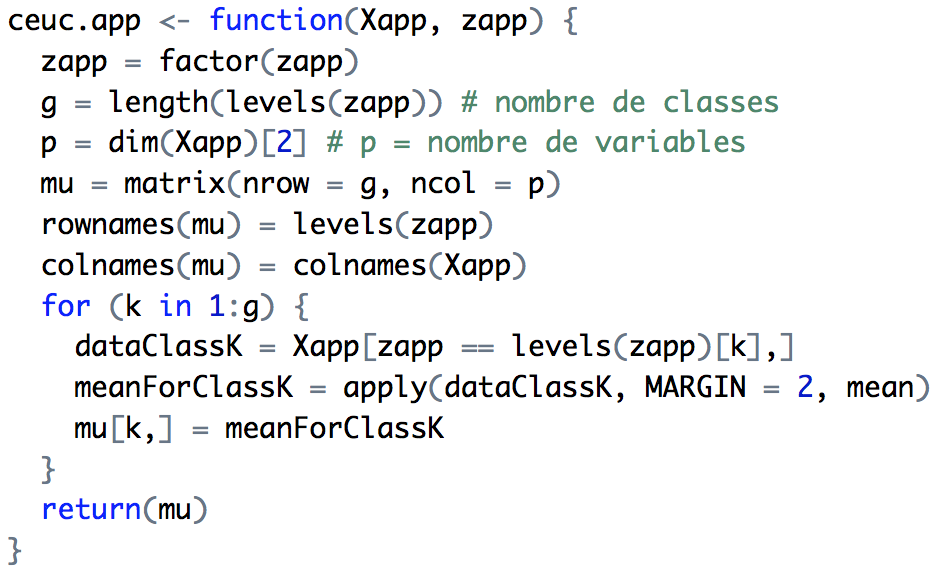
\includegraphics[width=.5\linewidth]{img/1-1-1-ceuc-app-code}
	\caption{\small Code de la fonction \texttt{ceuc.app()}}	
	\label{fig:1-1-1-ceuc-app-code}%
\end{figure}






\subsubsection{Fonction \texttt{ceuc.val()}~: discrimination d'un ensemble de données}

\begin{itemize}
	\item Objectif~:
	\begin{itemize}
		\item Classer un ensemble de données grâce au classifieur Euclidien.
	\end{itemize}
	
	\item Paramètres en entrée~:
	\begin{itemize}
		\item \texttt{mu}~: les paramètres du classifieur Euclidien, de taille $g \times p$~;
		\item \texttt{Xtst}~: les données de test à étiqueter~;
	\end{itemize}
	
	\item Algorithme~:
	\begin{itemize}
		\item Pour chaque individu $x$ des données de test \texttt{Xtst}~:
		\begin{itemize}
			\item Calculer les distances de $x$ aux centres de gravité de chaque classe~;
			\item Affecter $x$ à la classe dont le centre de gravité est le plus proche.
		\end{itemize}
	\end{itemize}
	\item Sortie~:
	\begin{itemize}
		\item Un vecteur d'étiquettes prédites pour les données de test \texttt{Xtst}.
	\end{itemize}
\end{itemize}

\begin{figure}[H]
	\centering
	\captionsetup{justification=centering, margin=4cm}
	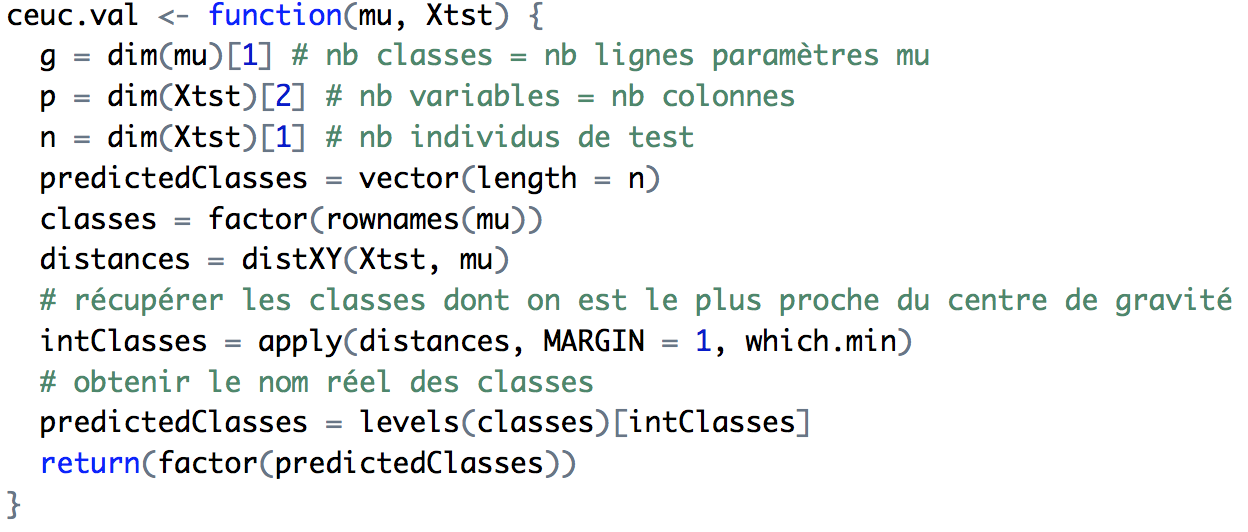
\includegraphics[width=.6\linewidth]{img/1-1-1-ceuc-val-code}
	\caption{\small Code de la fonction \texttt{ceuc.val()}}	
	\label{fig:1-1-1-ceuc-val-code}%
\end{figure}




\subsection{$K$ plus proches voisins}


\subsubsection{Fonction \texttt{kppv.val()}~: discrimination d'un ensemble de données}

\begin{itemize}
	\item Objectif~:
	\begin{itemize}
		\item Classer un ensemble de données grâce au classifieur des $K$ plus proches voisins.
	\end{itemize}
	
	\item Paramètres en entrée~:
	\begin{itemize}
		\item \texttt{Xapp}~: les données d'apprentissage~;
		\item \texttt{zapp}~: les étiquettes des données d'apprentissage~;
		\item \texttt{K}~: le nombre de voisins~;
		\item \texttt{Xtst}~: les données de test à étiqueter.
	\end{itemize}

	\item Algorithme~:
	\begin{itemize}
		\item Calculer les distances euclidiennes entre les individus \texttt{Xapp} et \texttt{Xtst}~;
		\item Pour chaque individu $x$ de \texttt{Xtst}~:
		\begin{itemize}
			\item Sélectionner les $K$ plus proches voisins de $x$~;
			\item Déterminer la classe $g$ la plus représentée parmi les $K$ plus proches voisins~;
			\item Affecter cette classe à $x$.
		\end{itemize}
	\end{itemize}

	\item Sortie~:
	\begin{itemize}
		\item Un vecteur d'étiquettes prédites pour les données de test \texttt{Xtst}.
	\end{itemize}
\end{itemize}
\begin{figure}[H]
	\centering
	\captionsetup{justification=centering, margin=4cm}
	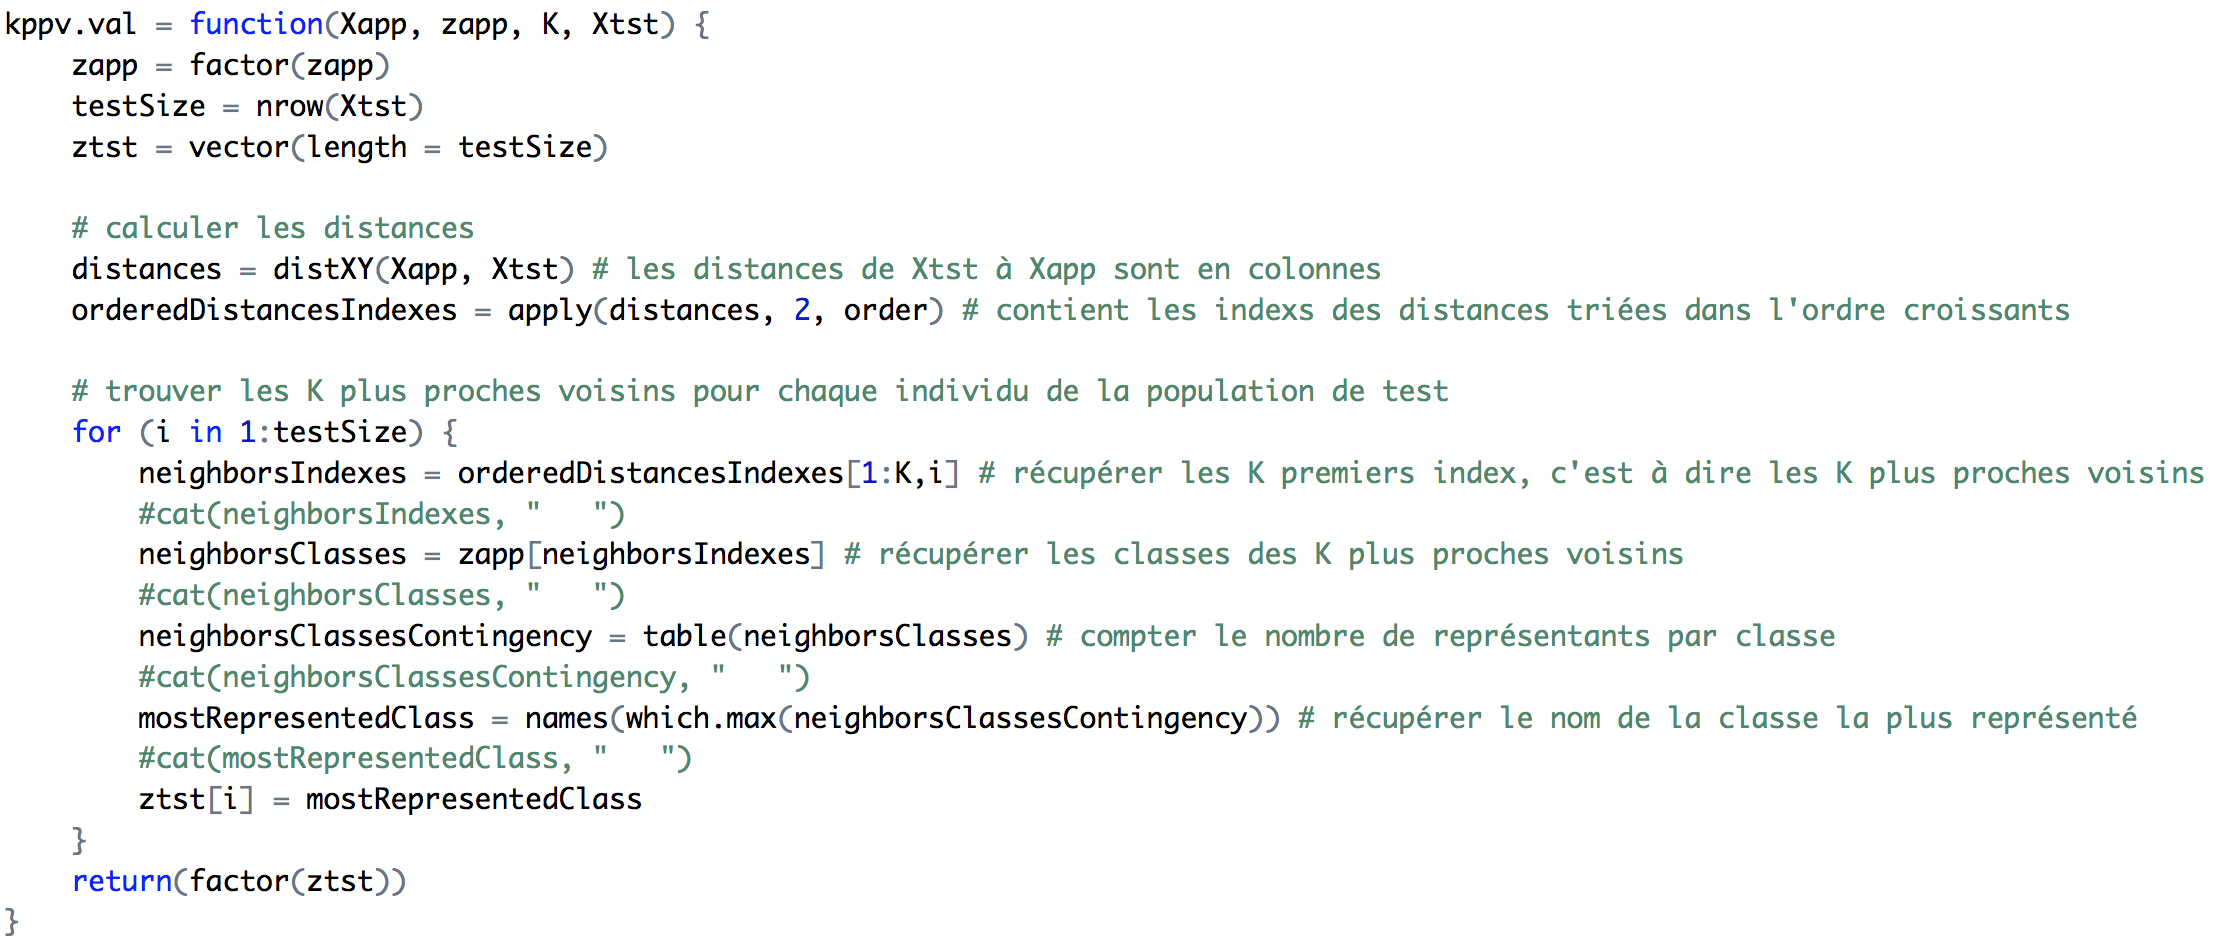
\includegraphics[width=.9\linewidth]{img/1-1-2-kppv-val-code}
	\caption{\small Code de la fonction \texttt{kppv.val()}}	
	\label{fig:1-1-2-kppv-val-code}%
\end{figure}


\subsubsection{Fonction \texttt{kppv.tune()}~: optimisation du nombre de voisins $K$}

\begin{itemize}
	\item Objectif~:
	\begin{itemize}
		\item Trouver le nombre $K$ optimal de voisins pour le classifieur des $K$ plus proches voisins.
	\end{itemize}
	
	\item Paramètres en entrée~:
	\begin{itemize}
		\item \texttt{Xapp}~: les données d'apprentissage~;
		\item \texttt{zapp}~: les étiquettes des données d'apprentissage~;
		\item \texttt{Xval}~: les données de validation~;
		\item \texttt{zval}~: les étiquettes des données de validation~~;
		\item \texttt{nppv}~: la liste des valeurs de $K$ à tester~;
		\item \texttt{skipOneNeighbor}~: si \texttt{VRAI}, ne prend pas en compte $K=1$ pour éviter le sur-apprentissage des données d'apprentissage.
		\item \texttt{useRandIndexes}~: si \texttt{VRAI}, utilise les indice de Rand afin de déterminer l'efficacité de la classification~; si \texttt{FAUX}, la proportion réelle d'étiquettes correctement prédites est utilisée pour calculer le taux de succès.
	\end{itemize}
	
	\item Algorithme~:
	\begin{itemize}
		\item Pour chaque valeur $k$ de la liste \texttt{nppv}~;
		\begin{itemize}
			\item Obtenir les étiquettes prédites grâce à la fonction \texttt{kppv.val()}~;
			\item Calculer le taux de succès de la discrimination grâce à la fonction \texttt{compute.sucess.rate()} (voir \autoref{annexe:compute.sucess.rate}) ou bien \texttt{adjustedRandIndex()}~;
			\item Si le taux de succès est égal au précédent, ajouter $k$ à la liste des $K$ optimum~;
			\item Sinon le taux de succès est supérieur au précédent, remplace la liste des $K$ optimum par $k$~;
			\item Sinon ne rien faire, le $k$ actuellement testé est moins efficace que le précédent~;
		\end{itemize}
	\end{itemize}
	
	\item Sortie~:
	\begin{itemize}
		\item Un vecteur contenants les valeurs des $K$ optimum (il peut y avoir plusieurs $K$ optimum).
	\end{itemize}
\end{itemize}

\begin{figure}[H]
	\centering
	\captionsetup{justification=centering, margin=4cm}
	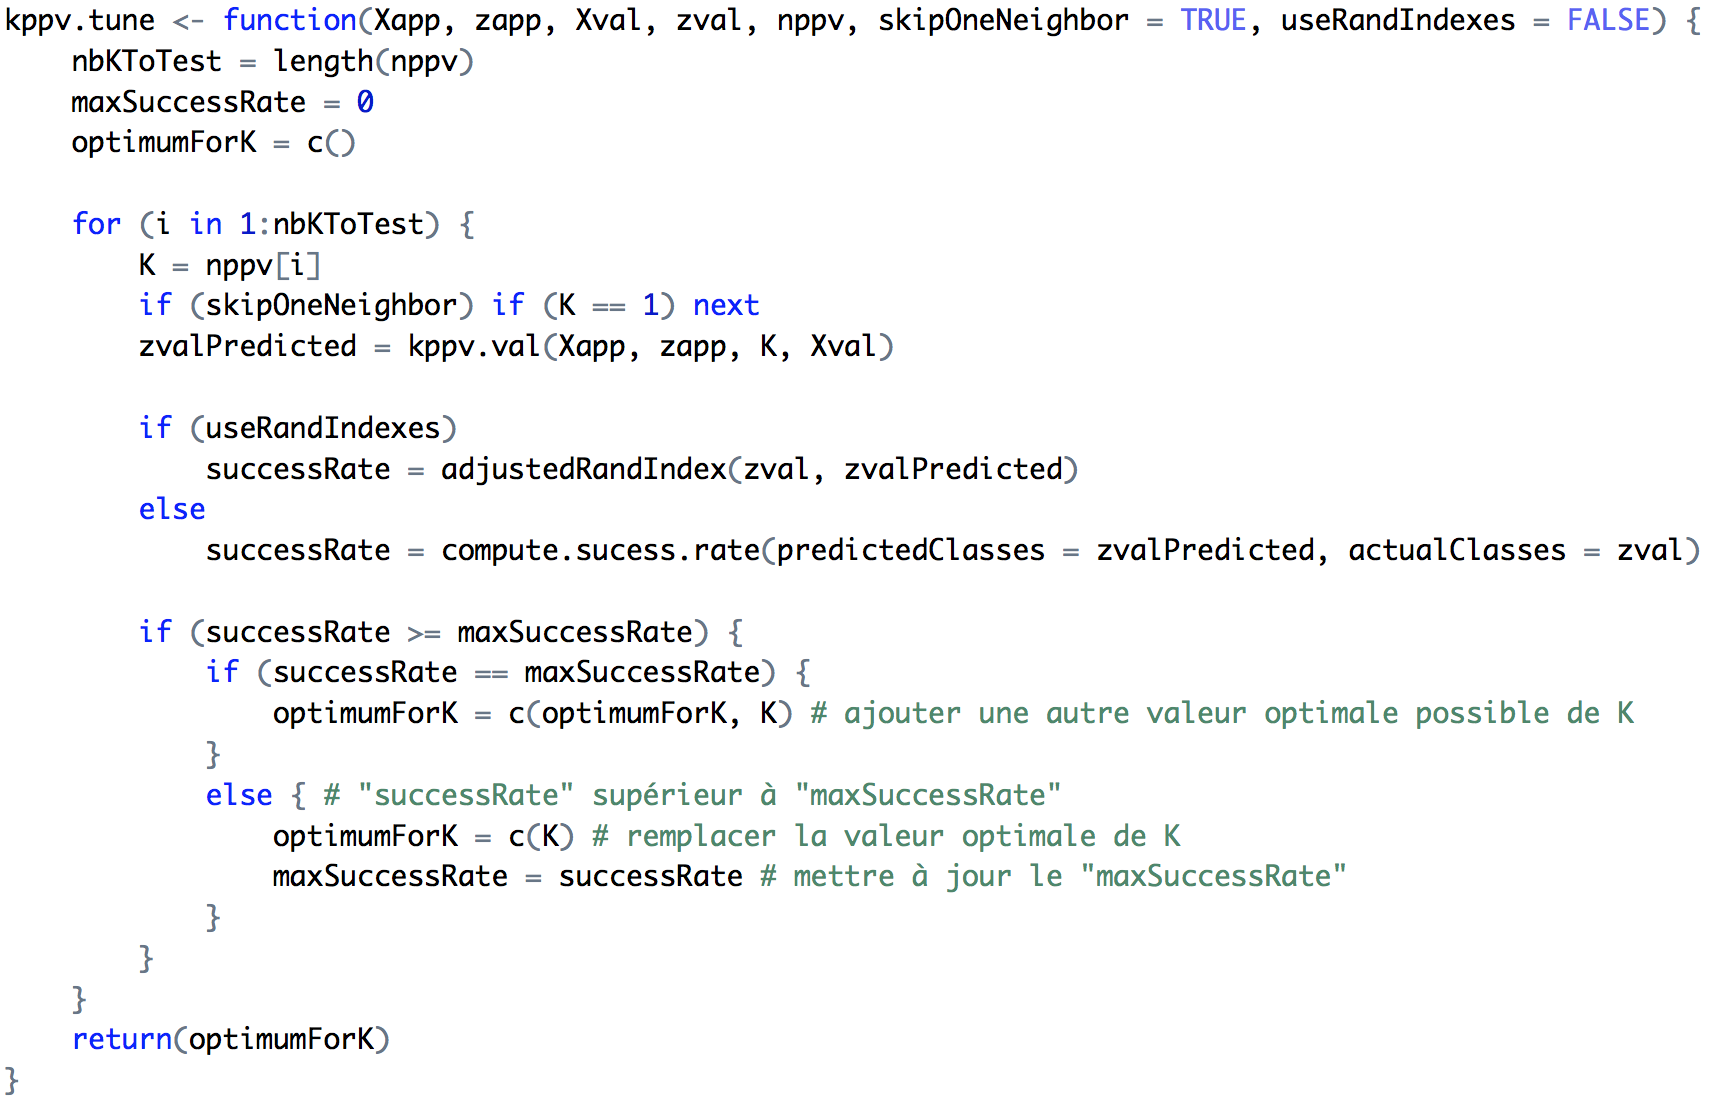
\includegraphics[width=.9\linewidth]{img/1-1-2-kppv-tune-code}
	\caption{\small Code de la fonction \texttt{kppv.tune()}}	
	\label{fig:1-1-2-kppv-tune-code}%
\end{figure}





\subsection{Test des fonctions}

\subsubsection{Classifieur Euclidien}


\begin{itemize}
	\item Données d'apprentissage~: fichier \textit{Synth1-1000.csv}~;
	\item Données d'affichage~: fichier \textit{Synth1-40.csv}.
\end{itemize}



\begin{figure}[H]
	\centering
	\captionsetup{justification=centering, margin=4cm}
	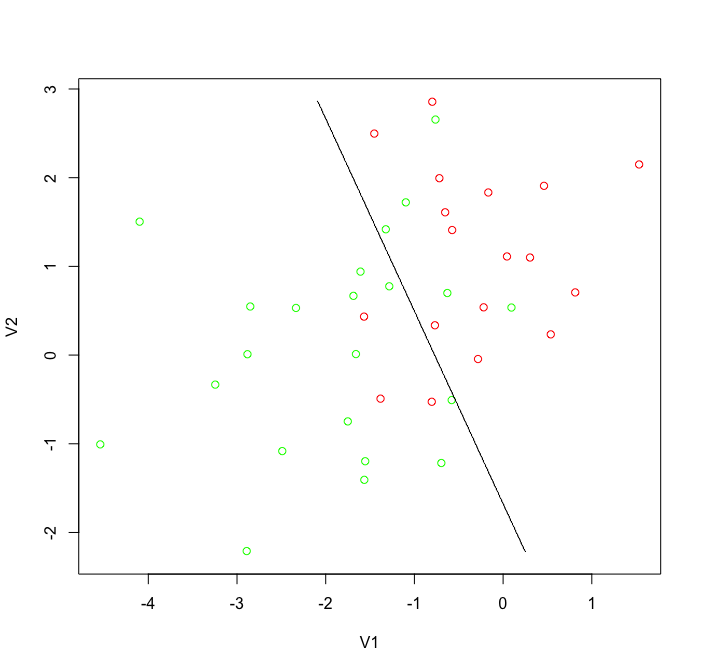
\includegraphics[width=.5\linewidth]{img/1-1-3-front-ceuc}
	\caption{\small Frontière de décision obtenue avec le classifieur Euclidien}	
	\label{fig:1-1-3-front-ceuc}%
\end{figure}


\begin{table}[H]
	\centering
	\begin{tabular}{r|rr}
		& V1 & V2 \\ 
		\hline
		\small Classe 1 & -0.01 & 0.92 \\ 
		\small Classe 2 & -1.96 & 0.02 \\ 
	\end{tabular}
	\caption{\small Coordonnées des centres de gravité des classes}
	\label{table:1-1-3-mu-class-euc}
\end{table}


\subsubsection{$K$ plus proches voisins}

\begin{itemize}
	\item Données d'apprentissage~: fichier \textit{Synth1-1000.csv}~;
	\item Données de validation~: fichier \textit{Synth1-500.csv}~;
	\item Données d'affichage~: fichier \textit{Synth1-40.csv}~;
	\item $K$ optimum trouvé~: 11.
\end{itemize}

\begin{figure}[H]
	\centering
	\captionsetup{justification=centering, margin=4cm}
	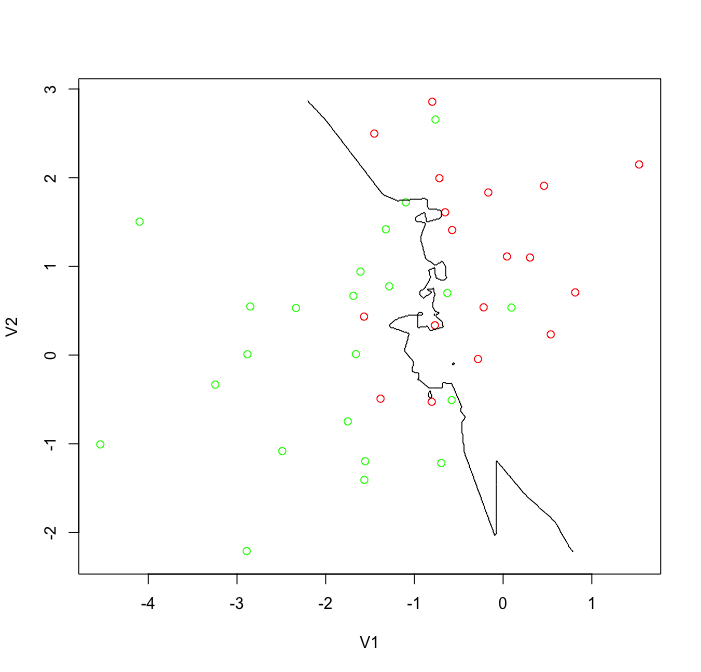
\includegraphics[width=.5\linewidth]{img/1-1-3-front-kppv}
	\caption{\small Frontière de décision obtenue avec le classifieur des $K$ plus proches voisins sur le jeu de données du fichier \textit{Synth1-40.csv}, avec $K optimum = 11$}
	\label{fig:1-1-3-front-kppv}%
\end{figure}






\section{Évaluation des performances}


On va ici évaluer et analyser le taux d'erreur $\epsilon$ des classifieurs.\\

Voici la procédure suivie pour chaque jeu de données, à répéter $N$ fois les actions suivantes~:
\begin{itemize}
	\item Séparer aléatoirement l’ensemble des données disponibles, de manière à former un ensemble d’apprentissage et un ensemble de test (et, de manière optionnelle, un ensemble de validation, s’il est nécessaire d’estimer un ou plusieurs hyper-paramètres, tel le nombre $K$ de voisins optimum pour le classifieur des $K$ plus proches voisins)~;
	\item Apprendre les paramètres du modèle sur l’ensemble d’apprentissage ainsi formé (après avoir éventuellement optimisé les hyper-paramètres sur l’ensemble de validation, s’il y a lieu), et calculer le taux d’erreur obtenu sur l’ensemble de test.
\end{itemize}

En déterminant de la sorte N séparations aléatoires de l’ensemble de données en un ensemble d’apprentissage et un ensemble de test, on peut ainsi recueillir un échantillon de $N$ estimations $E_{1},...,E_{N}$ du taux d’erreur (généralement effectuées sur l’ensemble de test). On peut alors déterminer une estimation ponctuelle $\hat{\epsilon} $ (moyenne) et un intervalle de confiance sur $\epsilon$.


\subsubsection{Notes sur les intervalles de confiances}
On suppose que l'échantillon $E$ constitué des $N$ estimations $E_{1},...,E_{N}$ du taux d’erreur est  \textit{\textbf{iid}}~:
\begin{itemize}
	\item Les $N$ observations peuvent être considérées comme indépendantes car les ensembles de test, d'apprentissage et de validation sont tirés de façon aléatoire~;
	\item Les $N$ observations sont identiquement distribuées car, quand bien même on ne connaît pas la loi des observations originelles ayant conduit à l'obtention des taux d'erreur, l'échantillon est constituée de moyennes, qui suivent par définition une loi gaussienne.
\end{itemize}

La variance étant inconnue, on peut alors approcher $\hat{\epsilon} = \overline{E}$ (l'espérance de l'échantillon) avec la loi de Student à $N-1$ degrés de liberté~:

\[
\sqrt{N} \times  \frac{\overline{E} - \epsilon}{\sigma^*} \sim S(N-1)
\]

Et donc l'intervalle de confiance est donné par~:

\[
IC(\epsilon) = [ \overline{E} - t_{1-\frac{\alpha}{2}} \frac{\sigma^*}{\sqrt{N}} , \overline{E} + t_{1-\frac{\alpha}{2}} \frac{\sigma^*}{\sqrt{N}}]
\]
où $t_{1-\frac{\alpha}{2}}$ est le fractile d'ordre $1-\frac{\alpha}{2}$ de la loi de Student à $N-1$ degrés de liberté.



\subsubsection{Notes sur l'analyse des résultats obtenus}

La démarche ici est d'analyser la bonne performance ou non d'un classifieur.\\

Le classifieur Euclidien, par exemple, est basé sur un modèle supposant que~:
\begin{itemize}
	\item Les classes possèdent la même dispersion~: les matrices $\Sigma$ sont communes à toutes les classes
	\item La dispersion des classes est spérique~: les matrices $\Sigma$ sont scalaires et diagonales
	\item Les classes ont toutes la même proportion égale à $\frac{1}{g}$
\end{itemize}

De plus, le classifieur étant Euclidien, il aura tendance à mieux marcher si les centres de gravité $\mu_{k}$ des classes sont éloignés entre eux que s'ils sont proches.\\


\subsection{Jeux de données \textit{Synth1-40}, \textit{Synth1-100}, \textit{Synth1-500} et \textit{Synth1-1000}}
\label{subsection:estimation-erreur-synth1}



\subsubsection{Estimation des paramètres}


\begin{table}[H]
	\centering
	\begin{tabular}{c|c|c|c}
		Fichier source & Centres de gravité $\mu$ & Variances $\Sigma$ & Proportions $\pi$ \\ 
		\hline
		\small Synth1-40 
		& 	$\mu_{1} = 
		\begin{pmatrix}
		-0.32 \\ 
		1.09
		\end{pmatrix} $ , 
		$\mu_{2} = 
		\begin{pmatrix}
		-1.88 \\ 
		0.11
		\end{pmatrix} $ 
		&  	$\Sigma_{1} = 
		\begin{pmatrix}
		0.68 & 0.12 \\
		0.12 & 1.01\\
		\end{pmatrix} $ , 
		$\Sigma_{2} = 
		\begin{pmatrix}
		1.38 & 0.32\\
		0.32 & 1.44 \\
		\end{pmatrix} $
		& 	$\begin{pmatrix} 
		\pi_{1} = 0.45\\
		\pi_{2} = 0.55
		\end{pmatrix}$\\ 
		\hline
		\small Synth1-100 
		& 	$\mu_{1} = 
		\begin{pmatrix}
		0.03 \\ 
		0.82
		\end{pmatrix} $ , 
		$\mu_{2} = 
		\begin{pmatrix}
		-1.97 \\ 
		-0.13
		\end{pmatrix} $ 
		&  	$\Sigma_{1} = 
		\begin{pmatrix}
		0.88 & -0.13\\
		-0.13 & 1.11\\
		\end{pmatrix} $ , 
		$\Sigma_{2} = 
		\begin{pmatrix}
		0.76 & -0.04\\
		-0.04 & 0.76\\
		\end{pmatrix} $
		& 	$\begin{pmatrix} 
		\pi_{1} = 0.54\\
		\pi_{2} = 0.46
		\end{pmatrix}$\\ 
		\hline
		\small Synth1-500 
		& 	$\mu_{1} = 
		\begin{pmatrix}
		0.13 \\ 
		0.88	
		\end{pmatrix} $ , 
		$\mu_{2} = 
		\begin{pmatrix}
		-1.88 \\ 
		-0.08
		\end{pmatrix} $ 
		&  	$\Sigma_{1} = 
		\begin{pmatrix}
		1.05 & 0.05\\
		0.05 & 0.98\\
		\end{pmatrix} $ , 
		$\Sigma_{2} = 
		\begin{pmatrix}
		0.97 & -0.11\\
		-0.11 & 0.98\\
		\end{pmatrix} $
		& 	$\begin{pmatrix} 
		\pi_{1} = 0.53\\
		\pi_{2} = 0.47
		\end{pmatrix}$\\ 
		\hline
		\small Synth1-1000 
		& 	$\mu_{1} = 
		\begin{pmatrix}
		-0.01 \\ 
		0.92
		\end{pmatrix} $ , 
		$\mu_{2} = 
		\begin{pmatrix}
		-1.96 \\ 
		0.02
		\end{pmatrix} $ 
		&  	$\Sigma_{1} = 
		\begin{pmatrix}
		0.97 & -0.07\\
		-0.07 & 1.08\\
		\end{pmatrix} $ , 
		$\Sigma_{2} = 
		\begin{pmatrix}
		0.99 & 0.02\\
		0.02 & 0.94\\
		\end{pmatrix} $
		&	 $\begin{pmatrix} 
		\pi_{1} = 0.5\\
		\pi_{2} = 0.5
		\end{pmatrix}$\\ 
	\end{tabular}
	\caption{\small Paramètres estimés des fichiers}
	\label{table:1-2-parametres-Synth1}
\end{table}


Plus on estime les paramètres sur un ensemble de données conséquent, plus ils se rapprochent des hypothèses du modèle Euclidien avec $\Sigma_{1} = \Sigma_{2}$ matrices diagonales et scalaires et $\pi_{1} = \pi_{2} = \frac{1}{g}$.

\subsubsection{Évaluation des performances du classifieur Euclidien}

Le tableau ci-dessous représente les estimations ponctuelle du taux d'erreur $\hat{\epsilon}$ et de l'intervalle de confiance sur $\epsilon$ (pour $\alpha = 0.05$) lors des discriminations effectuées avec le classifieur Euclidien. Ces mesures sont obtenues à partir d'un échantillon de $N = 20$ séparations aléatoires des jeux de données en ensembles d'apprentissage et de test.

\begin{table}[H]
	\centering
	\captionsetup{justification=centering, margin=4cm}
	\begin{tabular}{c|c|c}
		Fichier source & Données d'apprentissage & Données de test \\ 
		\hline
		\small Synth1-40 & $ \hat{\epsilon} = 0.206 $  &  $ \hat{\epsilon} = 0.242 $ \\
						&  $ IC(\epsilon) = [ 0.18 , 0.231 ] $  & $ IC(\epsilon) = [ 0.19 , 0.295 ] $ \\ 
		\hline
		\small Synth1-100 & $ \hat{\epsilon} = 0.093 $  &  $ \hat{\epsilon} = 0.083 $ \\
		&  $ IC(\epsilon) = [ 0.083 , 0.103 ] $  & $ IC(\epsilon) = [ 0.062 , 0.104 ] $ \\ 
		\hline
		\small Synth1-500 & $ \hat{\epsilon} = 0.127 $  &  $ \hat{\epsilon} = 0.146 $ \\
		&  $ IC(\epsilon) = [ 0.121 , 0.133 ] $  & $ IC(\epsilon) = [ 0.134 , 0.158 ] $ \\ 
		\hline
		\small Synth1-1000 & $ \hat{\epsilon} = 0.143 $  &  $ \hat{\epsilon} = 0.142 $ \\
		&  $ IC(\epsilon) = [ 0.139 , 0.148 ] $  & $ IC(\epsilon) = [ 0.135 , 0.15 ] $ \\ 
	\end{tabular}
	\caption{\small Estimation du taux d'erreur $\hat{\epsilon}$ et de l'intervalle de confiance sur $\epsilon$ pour $N = 20$ avec le classifieur Euclidien}
	\label{table:1-2-error-rate-Synth1-N-20-ceuc}
\end{table}



On observe plusieurs choses~:
\begin{itemize}
	\item Variation du taux d'erreur $\hat{\epsilon}$ entre les données d'apprentissage et de test
	\begin{itemize}
		\item Parfois $\hat{\epsilon}_{app} < \hat{\epsilon}_{test}$ et parfois c'est l'inverse, $\hat{\epsilon}_{test} < \hat{\epsilon}_{app}$~;
		\item Cela dépend fortement des tirages des données d'apprentissage et de test qui sont aléatoires.
		\item Sans tirer de conclusions, on peut supposer qu'avoir $\hat{\epsilon}_{app} < \hat{\epsilon}_{test}$ signale un sur-apprentissage, les centres de gravité des données d'apprentissage n'étant pas particulièrement représentatifs des centres de gravité des données de test~;
	\end{itemize}
	\item Étendue des intervalles de confiance
	\begin{itemize}
		\item L'étendue des intervalles de confiance sur ${\epsilon}_{app}$ est systématiquement plus réduite que celle des intervalles de confiance sur sur ${\epsilon}_{test}$~;
		\item L'apprentissage des paramètres du modèle se fait sur les données d'apprentissage, il est donc logique que l'écart-type de $\hat{\epsilon}_{app}$ (racine carré de la dispersion du taux d'erreur autour de son espérance) soit plus petit que celui de $\hat{\epsilon}_{test}$~;
		\item Ainsi, la valeur $\sigma^*/\sqrt{N}$ sera inférieure pour les données d'apprentissage, et donc l'étendue de l'intervalle de confiance ($t_{1-\alpha/2} \times \sigma^*/\sqrt{N}$) sera plus petite.
	\end{itemize}
	\item Non corrélation apparente de la taille des jeux de données et des taux d'erreurs
	\begin{itemize}
		\item Selon toute logique, plus le jeu de données est conséquent, plus le taux d'erreur devrait diminuer et converger vers le taux d'erreur de Bayes~;
		\item Néanmoins, on peut toujours observer un taux d'erreur inférieur à celui de Bayes, tout dépend du jeu de données en question~: s'il ne contient que deux points très éloignés, on aura par exemple un taux d'erreur nul~;
		\item Cas du fichier "\textit{Synth1-100}"
		\begin{itemize}
			\item Ce fichier présente une estimation du taux d'erreur très faible par rapport aux autres, et il en va de même pour son intervalle de confiance~;
			\item Cela s'explique par les dispersions des deux classes, et plus particulièrement par celle de la classe numéro deux avec deux variances égales à 0.76~;
			\item La zone de mélange entre les deux classes et donc très réduite, d'où le faible taux d'erreur.
		\end{itemize}
	\end{itemize}
\end{itemize}





\subsubsection{Classifieur des $K$ plus proches voisins et sur-apprentissage}

On cherche ici déterminer le nombre optimal de voisins à l’aide de la fonction \texttt{kppv.tune()}, en utilisant l’ensemble d’apprentissage comme ensemble de validation.

On obtient $K = 1$, car on fait du sur-apprentissage. Le plus proche voisin d'un point étant lui-même, le taux de succès de la classification est de 100\% pour $K=1$.

\subsubsection{Évaluation des performances du classifieur des $K$ plus proches voisins}

Le tableau ci-dessous représente les estimations ponctuelle du taux d'erreur $\hat{\epsilon}$ et de l'intervalle de confiance sur $\epsilon$ (pour $\alpha = 0.05$) lors des discriminations effectuées avec le classifieur des $K$ plus proches voisins. Ces mesures sont obtenues à partir d'un échantillon de $N = 20$ séparations aléatoires des jeux de données en ensembles d'apprentissage et de test.

\begin{table}[H]
	\centering
	\captionsetup{justification=centering, margin=4cm}
	\begin{tabular}{c|c|c}
		Fichier source & Données d'apprentissage & Données de test \\ 
		\hline
		\small Synth1-40 & $ \hat{\epsilon} = 0.19 $  &  $ \hat{\epsilon} = 0.27 $ \\
		&  $ IC(\epsilon) = [ 0.157 , 0.223 ] $  & $ IC(\epsilon) = [ 0.219 , 0.321 ] $ \\ 
		\hline
		\small Synth1-100 & $ \hat{\epsilon} = 0.090 $  &  $ \hat{\epsilon} = 0.112 $ \\
		&  $ IC(\epsilon) = [ 0.072 , 0.108 ] $  & $ IC(\epsilon) = [ 0.081 , 0.144 ] $ \\ 
		\hline
		\small Synth1-500 & $ \hat{\epsilon} = 0.122 $  &  $ \hat{\epsilon} = 0.146 $ \\
		&  $ IC(\epsilon) = [ 0.115 , 0.129 ] $  & $ IC(\epsilon) = [ 0.133 , 0.158 ] $ \\ 
		\hline
		\small Synth1-1000 & $ \hat{\epsilon} = 0.126 $  &  $ \hat{\epsilon} = 0.160 $ \\
		&  $ IC(\epsilon) = [ 0.119 , 0.133 ] $  & $ IC(\epsilon) = [ 0.15 , 0.169 ] $ \\ 
	\end{tabular}
	\caption{\small Estimation du taux d'erreur $\hat{\epsilon}$ et de l'intervalle de confiance sur $\epsilon$ pour $N = 20$ avec le classifieur des $K$ plus proches voisins}
	\label{table:1-2-error-rate-Synth1-N-20-kppv}
\end{table}



Comparaison avec le classifieur Euclidien~:
\begin{itemize}
	\item Le classifieur des $K$ plus proches voisins obtient de meilleurs résultats que le classifieur Euclidien sur les données d'apprentissage~;
	\item Il est par contre moins efficace que le classifieur Euclidien sur les données de test.
\end{itemize}

D'après l'estimation des paramètres, les données ont été générées de manière à respecter les hypothèses du classifieur Euclidien. Il est donc logique que ce dernier soit plus efficace sur les données de test. De plus, le fait d'avoir la même dispersion dans les deux classes peut pénaliser le travail du classifieur des $K$ plus proches voisins~: plus la dispersion d'une classe est faible, plus ses voisins sont proches et donc plus discrimination pourra être efficace pour cette classe.
Enfin, notons que le classifieur des K plus proches voisins ne suit pas un modèle~: il se base complètement sur les données d'apprentissage pour discriminer les données de test. Si ces dernières ne sont pas représentatives, alors la classification aura un fort taux d'échec.








\subsection{Jeux de données \textit{Synth2-1000}}
\label{subsection:estimation-erreur-synth2}
\subsubsection{Estimation des paramètres}


\begin{table}[H]
	\centering
	\begin{tabular}{c|c|c|c}
		Fichier source & Centres de gravité $\mu$ & Variances $\Sigma$ & Proportions $\pi$ \\ 
		\hline
		\small Synth2-1000 
		& 	$\mu_{1} = 
		\begin{pmatrix}
		3.02 \\ 
		-0.01
		\end{pmatrix} $ , 
		$\mu_{2} = 
		\begin{pmatrix}
		-2.14 \\ 
		-0.03
		\end{pmatrix} $ 
		&  	$\Sigma_{1} = 
		\begin{pmatrix}
		0.99 & 0.11 \\
		0.11 & 1.09\\
		\end{pmatrix} $ , 
		$\Sigma_{2} = 
		\begin{pmatrix}
		4.43 & -0.15\\
		-0.15 & 1.03 \\
		\end{pmatrix} $
		& 	$\begin{pmatrix} 
		\pi_{1} = 0.52\\
		\pi_{2} = 0.48
		\end{pmatrix}$\\ 
	\end{tabular}
	\caption{\small Paramètres estimés du fichier "\textit{Synth2-1000}"}
	\label{table:1-2-parametres-Synth2}
\end{table}



Paramètres estimés versus modèle du classifieur Euclidien~:
\begin{itemize}
	\item Ces données semblent ne respecter que la condition d'égalité des proportions du modèle du classifieur Euclidien~;
	\item Seule la classe 1 possède une matrice de variance scalaire et diagonale (les termes non diagonaux ont des valeurs négligeables)~;
	\item Les $\Sigma_k$ ne sont pas égales entre-elles~: les classes n'ont pas la même dispersion.
\end{itemize}


Le classifieur Euclidien semblerait donc à première vue déconseillé. Par contre, on remarque que les centres de gravité sont à la fois alignés particulièrement éloignés et que la dispersion des classes définit une surface de chevauchement faible.
Dans les faits, il est donc fort probable que le classifieur Euclidien soit efficace.

De même pour le classifieur des $K$ plus proches voisins qui sera lui aussi vraisemblablement efficace. En raison de la faible surface de chevauchement et de la différence de dispersion, il y aura beaucoup plus de voisins de la classe 1 au 
sein de la zone de chevauchement que de voisin de classe 2.\\



Voici une représentation graphique des deux classes~:
\begin{figure}[H]
	\centering
	\captionsetup{justification=centering, margin=4cm}
	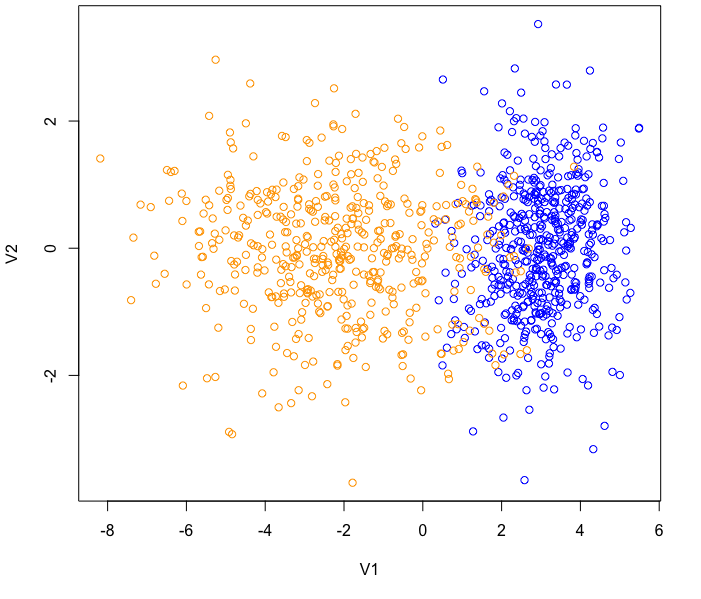
\includegraphics[width=.6\linewidth]{img/1-2-2-plot-Synth2-1000}
	\caption{\small Représentation graphique des données du fichier "\textit{Synth2-1000}" en fonction des classes 1 et 2}	
	\label{fig:1-2-2-plot-Synth2-1000}%
\end{figure}





\subsubsection{Performances des classifieurs Euclidien et des $K$ plus proches voisins}


\begin{table}[H]
	\centering
	\captionsetup{justification=centering, margin=4cm}
	\begin{tabular}{c|c|c}
		Fichier source & Données d'apprentissage & Données de test \\ 
		\hline
		\small Synth2-1000 & $ \hat{\epsilon} = 0.062 $  &  $ \hat{\epsilon} = 0.063 $ \\
		&  $ IC(\epsilon) = [ 0.061 , 0.064 ] $  & $ IC(\epsilon) = [ 0.059 , 0.067 ] $ \\ 
	\end{tabular}
	\caption{\small Estimation du taux d'erreur $\hat{\epsilon}$ et de l'intervalle de confiance sur $\epsilon$ pour $N = 20$ avec le classifieur Euclidien}
	\label{table:1-2-error-rate-Synth2-N-20-ceuc}
\end{table}


\begin{table}[H]
	\centering
	\captionsetup{justification=centering, margin=4cm}
	\begin{tabular}{c|c|c}
		Fichier source & Données d'apprentissage & Données de test \\ 
		\hline
		\small Synth2-1000 & $ \hat{\epsilon} = 0.052 $  &  $ \hat{\epsilon} = 0.061 $ \\
		&  $ IC(\epsilon) = [ 0.049 , 0.055 ] $  & $ IC(\epsilon) = [ 0.056 , 0.066 ] $ \\ 
	\end{tabular}
	\caption{\small Estimation du taux d'erreur $\hat{\epsilon}$ et de l'intervalle de confiance sur $\epsilon$ pour $N = 20$ avec le classifieur des $K$ plus proches voisins}
	\label{table:1-2-error-rate-Synth2-N-20-kppv}
\end{table}



Comme supposé à la vue des estimations des paramètres, les deux classifieurs sont très efficace, avec moins de 7\% d'erreur.\\

Le classifieur Euclidien est assez stable, avec des taux d'erreur quasiment identiques entre les données d'apprentissage et de test.\\

Le classifieur des $K$ plus proches voisins est encore une fois meilleur sur les données d'apprentissage que sur les données de test. Il est aussi légèrement plus efficace que le classifieur Euclidien, mais à peine. C'est surement du à sa capacité à mieux discriminer les individus au sein de la zone de chevauchement, en raison des différences de dispersion entre les classes.\\

Voici les frontières de décision obtenues sur les données de test une séparation aléatoire~:

\begin{figure}[H]
	\centering
	\captionsetup{justification=centering, margin=2cm}
	\begin{subfigure}[b]{0.5\linewidth}
		\centering
		\captionsetup{justification=centering, margin=1cm}
		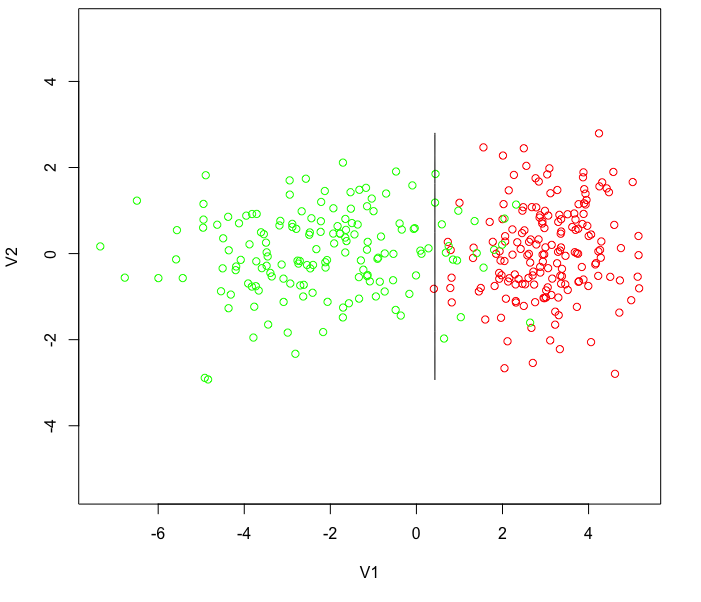
\includegraphics[width=1\linewidth]{img/1-2-2-Synth2-1000-front-euc}
		\caption{\small Classifieur Euclidien}
	\end{subfigure}%
	\begin{subfigure}[b]{0.5\linewidth}
		\centering
		\captionsetup{justification=centering, margin=1cm}
		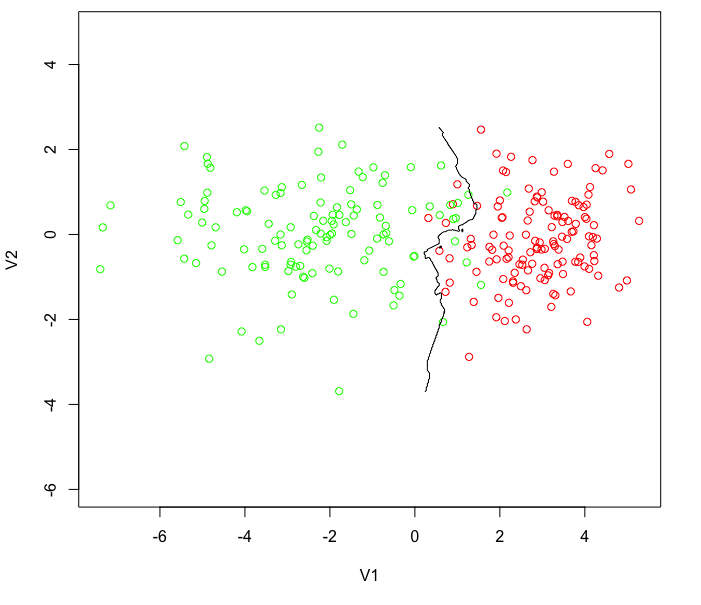
\includegraphics[width=1\linewidth]{img/1-2-2-Synth2-1000-front-kppv}
		\caption{\small Classifieur des $K$ plus proches voisins}
	\end{subfigure}%
	\caption{\small Frontières de décision pour le fichier "\textit{Synth2-1000}"}
	\label{fig:1-2-2-Synth2-1000-frontiere-decision}%
\end{figure}





\subsection{Jeux de données réelles}




\subsubsection{Taux d'erreur et intervalles de confiances}

\textbf{Classifieur Euclidien}

\begin{table}[H]
	\centering
	\captionsetup{justification=centering, margin=4cm}
	\begin{tabular}{c|c|c}
		Fichier source & Données d'apprentissage & Données de test \\ 
		\hline
		\small Breastcancer & $ \hat{\epsilon} = 0.037 $  &  $ \hat{\epsilon} = 0.043 $ \\
		&  $ IC(\epsilon) = [ 0.035 , 0.039 ] $  & $ IC(\epsilon) = [ 0.038 , 0.048 ] $ \\ 
		\hline
		\small Pima & $ \hat{\epsilon} = 0.243 $  &  $ \hat{\epsilon} = 0.254 $ \\
		&  $ IC(\epsilon) = [ 0.235 , 0.25 ] $  & $ IC(\epsilon) = [ 0.242 , 0.267 ] $ \\ 
	\end{tabular}
	\caption{\small Estimation du taux d'erreur $\hat{\epsilon}$ et de l'intervalle de confiance sur $\epsilon$ pour $N = 20$ avec le classifieur Euclidien}
	\label{table:1-2-3-error-rate-ceuc}
\end{table}


\textbf{Classifieur des $K$ plus proches voisins}

\begin{table}[H]
	\centering
	\captionsetup{justification=centering, margin=4cm}
	\begin{tabular}{c|c|c}
		Fichier source & Données d'apprentissage & Données de test \\ 
		\hline
		\small Breastcancer & $ \hat{\epsilon} = 0.020 $  &  $ \hat{\epsilon} = 0.042 $ \\
		&  $ IC(\epsilon) = [ 0.017 , 0.024 ] $  & $ IC(\epsilon) = [ 0.036 , 0.048 ] $ \\ 
		\hline
		\small Pima & $ \hat{\epsilon} = 0.188 $  &  $ \hat{\epsilon} = 0.265 $ \\
		&  $ IC(\epsilon) = [ 0.174 , 0.201 ] $  & $ IC(\epsilon) = [ 0.253 , 0.277 ] $ \\ 
	\end{tabular}
	\caption{\small Estimation du taux d'erreur $\hat{\epsilon}$ et de l'intervalle de confiance sur $\epsilon$ pour $N = 20$ avec le classifieur des $K$ plus proches voisins}
	\label{table:1-2-3-error-rate-kppv}
\end{table}


De toute évidence, la discrimination sur les données \textit{Breastcancer} est très efficace, que ce soit avec le classifieur Euclidien ou celui des $K$ plus proches voisins. Par contre pour ce qui est des données \textit{Pima} le taux d'erreur avoisine les 25\% en moyenne. 75\% de chance de trouver juste est déjà bien, mais ce n'est pas fiable.


\subsubsection{Possible explication grâce aux estimations des paramètres}

\textbf{Données \textit{Breastcancer}}~:

\begin{table}[H]
	\centering
	\begin{tabular}{r|rrrrrrrrr}
		& V2 & V3 & V4 & V5 & V6 & V7 & V8 & V9 & V10 \\ 
		\hline
		$\mu_{1}$ & 2.96 & 1.31 & 1.41 & 1.35 & 2.11 & 2.41 & 2.08 & 1.26 & 1.07 \\ 
		$\mu_{2}$ & 7.19 & 6.58 & 6.56 & 5.59 & 5.33 & 4.71 & 5.97 & 5.86 & 2.60 \\ 
	\end{tabular}
	\caption{Breastcancer~: Centre de gravité des classes}
\end{table}
\begin{table}[H]
	\centering
	\begin{tabular}{r|r}
		& Proportions \\ 
		\hline
		$\pi_{1}$ & 0.65 \\ 
		$\pi_{2}$ & 0.35 \\ 
	\end{tabular}
	\caption{Breastcancer~: Proportions des classes}
\end{table}
\begin{table}[H]
	\centering
	\begin{tabular}{r|rrrrrrrrr}
		& V2 & V3 & V4 & V5 & V6 & V7 & V8 & V9 & V10 \\ 
		\hline
		V2 & \textbf{2.80} & 0.39 & 0.48 & 0.39 & 0.23 & 0.21 & 0.18 & 0.33 & -0.03 \\ 
		V3 & 0.39 & \textbf{0.73} & 0.57 & 0.22 & 0.31 & 0.48 & 0.24 & 0.40 & 0.02 \\ 
		V4 & 0.48 & 0.57 & \textbf{0.92} & 0.21 & 0.29 & 0.41 & 0.20 & 0.36 & -0.00 \\ 
		V5 & 0.39 & 0.22 & 0.21 & \textbf{0.84} & 0.24 & 0.35 & 0.11 & 0.22 & 0.03 \\ 
		V6 & 0.23 & 0.31 & 0.29 & 0.24 & \textbf{0.77} & 0.30 & 0.14 & 0.37 & -0.01 \\ 
		V7 & 0.21 & 0.48 & 0.41 & 0.35 & 0.30 & \textbf{1.49} & 0.28 & 0.34 & 0.05 \\ 
		V8 & 0.18 & 0.24 & 0.20 & 0.11 & 0.14 & 0.28 & \textbf{1.13} & 0.35 & -0.02 \\ 
		V9 & 0.33 & 0.40 & 0.36 & 0.22 & 0.37 & 0.34 & 0.35 & \textbf{0.91} & 0.03 \\ 
		V10 & -0.03 & 0.02 & -0.00 & 0.03 & -0.01 & 0.05 & -0.02 & 0.03 & \textbf{0.26} \\ 
	\end{tabular}
	\caption{Breastcancer~: Matrice de covariance $\Sigma_{1}$}
\end{table}

\begin{table}[H]
	\centering
	\begin{tabular}{r|rrrrrrrrr}
		& V2 & V3 & V4 & V5 & V6 & V7 & V8 & V9 & V10 \\ 
		\hline
		V2 & \textbf{5.94} & 0.65 & 0.70 & -1.12 & 0.10 & -0.42 & -0.10 & -0.11 & 0.74 \\ 
		V3 & 0.65 & \textbf{7.42} & 5.04 & 2.79 & 3.07 & -0.41 & 2.42 & 2.73 & 1.68 \\ 
		V4 & 0.70 & 5.04 & \textbf{6.60} & 2.20 & 2.40 & -0.25 & 1.98 & 2.66 & 1.38 \\ 
		V5 & -1.12 & 2.79 & 2.20 & \textbf{10.22} & 1.51 & -1.74 & 2.46 & 1.98 & 1.65 \\ 
		V6 & 0.10 & 3.07 & 2.40 & 1.51 & \textbf{5.97} & -0.25 & 1.21 & 1.89 & 2.09 \\ 
		V7 & -0.42 & -0.41 & -0.25 & -1.74 & -0.25 & \textbf{7.06} & -0.61 & 0.34 & 0.03 \\ 
		V8 & -0.10 & 2.42 & 1.98 & 2.46 & 1.21 & -0.61 & \textbf{5.21} & 1.94 & 0.35 \\ 
		V9 & -0.11 & 2.73 & 2.66 & 1.98 & 1.89 & 0.34 & 1.94 & \textbf{11.21} & 1.91 \\ 
		V10 & 0.74 & 1.68 & 1.38 & 1.65 & 2.09 & 0.03 & 0.35 & 1.91 & \textbf{6.58} \\ 
	\end{tabular}
	\caption{Breastcancer~: Matrice de covariance $\Sigma_{2}$}
\end{table}



On remarque deux choses qui peuvent expliquer la bonne discrimination euclidienne et des $K$ plus proches voisins~:
\begin{itemize}
	\item Les différences de valeurs entre les coordonnées des centres de gravité des classes
	\begin{itemize}
		\item Toutes les coordonnées sont positives mais les coordonnées de la classe 2 sont deux à trois fois plus élevées~;
		\item On peut donc en conclure que les centres de gravité des classes sont éloignés.
	\end{itemize}
	\item Les différences de valeurs des dispersions des classes sur chaque axe (variables V1,...,V10)
	\begin{itemize}
		\item La classe n°1 semble très peu dispersée et d'une forme assez sphérique. Seules les variances des variables V1 et V10.
		\item Comparativement, la dispersion de la seconde classe est beaucoup plus importante avec un minimum de 5.21 pour V8	et un maximum de 11.21 pour V9.
	\end{itemize}
\end{itemize}

En conclusion, on peut s'attendre à une très faible zone de chevauchement ainsi qu'à une classe légèrement sphérique et concentrée et une autre moins sphérique et plus dispersée.\\
~\\







\textbf{Données \textit{Pima}}~:

\begin{table}[H]
	\centering
	\begin{tabular}{r|rrrrrrr}
		& npreg & glu & bp & skin & bmi & ped & age \\ 
		\hline
		$\mu_{1}$  & 2.93 & 110.02 & 69.91 & 27.29 & 31.43 & 0.45 & 29.22 \\ 
		$\mu_{2}$  & 4.70 & 143.12 & 74.70 & 32.98 & 35.82 & 0.62 & 36.41 \\ 
	\end{tabular}
	\caption{Pima~: Centre de gravité des classes}
\end{table}

\begin{table}[H]
	\centering
	\begin{tabular}{rr}
		\hline
		& Proportions \\ 
		\hline
		$\pi_{1}$ & 0.67 \\ 
		$\pi_{2}$ & 0.33 \\ 
	\end{tabular}
	\caption{Pima~: Proportions des classes}
\end{table}

\begin{table}[H]
	\centering
	\begin{tabular}{r|rrrrrrr}
		& npreg & glu & bp & skin & bmi & ped & age \\ 
		\hline
		npreg & \textbf{7.77} & 4.62 & 6.63 & 3.67 & 0.01 & -0.04 & 18.30 \\ 
		glu & 4.62 & \textbf{589.85} & 56.25 & 32.57 & 25.48 & 0.66 & 42.91 \\ 
		bp & 6.63 & 56.25 & \textbf{141.68} & 28.70 & 23.08 & -0.13 & 39.42 \\ 
		skin & 3.67 & 32.57 & 28.70 & \textbf{101.61} & 44.32 & 0.06 & 17.46 \\ 
		bmi & 0.01 & 25.48 & 23.08 & 44.32 & \textbf{42.86} & 0.09 & 4.47 \\ 
		ped & -0.04 & 0.66 & -0.13 & 0.06 & 0.09 & \textbf{0.09} & 0.06 \\ 
		age & 18.30 & 42.91 & 39.42 & 17.46 & 4.47 & 0.06 & \textbf{98.08} \\ 
	\end{tabular}
	\caption{Pima~: Matrice de covariance $\Sigma_{1}$}
\end{table}

\begin{table}[H]
	\centering
	\begin{tabular}{r|rrrrrrr}
		& npreg & glu & bp & skin & bmi & ped & age \\ 
		\hline
		npreg & \textbf{15.36} & -9.87 & 6.14 & -4.14 & -4.65 & -0.09 & 23.53 \\ 
		glu & -9.87 & \textbf{977.50} & 32.84 & 31.18 & 10.24 & 0.23 & 34.69 \\ 
		bp & 6.14 & 32.84 & \textbf{156.85} & 12.36 & 18.01 & -0.18 & 36.27 \\ 
		skin & -4.14 & 31.18 & 12.36 & \textbf{108.06} & 35.55 & 0.54 & -7.44 \\ 
		bmi & -4.65 & 10.24 & 18.01 & 35.55 & \textbf{43.71} & 0.39 & -13.77 \\ 
		ped & -0.09 & 0.23 & -0.18 & 0.54 & 0.39 & \textbf{0.16} & -0.15 \\ 
		age & 23.53 & 34.69 & 36.27 & -7.44 & -13.77 & -0.15 & \textbf{117.45} \\ 
	\end{tabular}
	\caption{Pima~: Matrice de covariance $\Sigma_{2}$}
\end{table}



On remarque deux choses qui peuvent expliquer la mauvaise discrimination euclidienne et des $K$ plus proches voisins~:
\begin{itemize}
	\item On n'observe pas de différences flagrantes entre les coordonnées des centres de gravité des classes, il se peut donc qu'ils soient relativement proches~;
	\item Valeurs des dispersions des classes
	\begin{itemize}
		\item Les classes ne sont absolument pas sphériques~;
		\item Elles ont par contre des dispersions qui sembles proches l'une de l'autres.
	\end{itemize}
\end{itemize}

En conclusion, on peut s'attendre à une zone de chevauchement conséquentes, les centres de gravité étant relativement proche. De plus, la dispersion étant elle aussi proche entre les classes, le classifieur des $K$ plus proches voisins ne sera pas beaucoup plus efficace que le classifieur Euclidien.












\chapter{Règle de Bayes}


\subsubsection{Explications sur l'obtention des jeux de données synthétiques}

Les jeux de données étudiés précédemment ont été obtenus de la manière suivante~:
\begin{itemize}
	\item Tout d’abord, l’effectif $n_1$ de la classe $\omega_1$ a été déterminé par tirage aléatoire suivant une loi binomiale de paramètres $n$ et $\pi_1 = 0.5$~;
	\item $n_1$ individus ont ensuite été générés dans la classe $\omega_1$ suivant une loi normale bivariée de paramètres $\mu_1$ et $\Sigma_{1}$, et $n_2 = n - n_1$ individus ont été générés dans la classe $\omega_2$ suivant une loi normale bivariée de paramètres $\mu_2$ et $\Sigma_{2}$.
\end{itemize}

Pour les jeux de données \textit{Synth1-$n$}, on a utilisé comme paramètres~:
\[
	\mu_1 = \begin{pmatrix} 0 \\ 1 \end{pmatrix}, 
	\quad \mu_2 = \begin{pmatrix} -2 \\ 0 \end{pmatrix},
	\quad \Sigma_1 = \Sigma_2 = \begin{pmatrix} 1 & 0 \\ 0 & 1 \end{pmatrix}
\]

Pour les jeux de données \textit{Synth2-$n$}, on a utilisé comme paramètres~:
\[
	\mu_1 = \begin{pmatrix} 3 \\ 0 \end{pmatrix}, 
	\quad \mu_2 = \begin{pmatrix} -2 \\ 0 \end{pmatrix},
	\quad \Sigma_1 = \begin{pmatrix} 1 & 0 \\ 0 & 1 \end{pmatrix}, 
	\quad \Sigma_2 = \begin{pmatrix} 5 & 0 \\ 0 & 1 \end{pmatrix}
\]




\section{Distribution marginales des variables $X^1$ et $X^2$}


Les données sont obtenues pour chaque classe en suivant une loi normale bi-variée~: 
\begin{align*}
	X_{\omega_1} \sim N_{p=2}(\mu_{\omega_1}, \Sigma_{\omega_1}) \\
	X_{\omega_2} \sim N_{p=2}(\mu_{\omega_2}, \Sigma_{\omega_2}) \\
\end{align*}

Une des propriétés nous dit que si $X \sim N_{p}(\mu, \Sigma)$ alors toutes les lois marginales et conditionnelles sont des lois normales.\\


Les variables $X^1$ et $X^2$ suivent donc de manière générale, pour chaque classe, les lois suivantes~:
\begin{align*}
X_{\omega_1}^1 &\sim N(\mu_{11}, \sigma_{11}^2) \\
X_{\omega_2}^1 &\sim N(\mu_{21}, \sigma_{21}^2)  \\
X_{\omega_1}^2 &\sim N(\mu_{12}, \sigma_{12}^2) \\
X_{\omega_2}^2 &\sim N(\mu_{22}, \sigma_{22}^2) 
\end{align*}
	

Lorsqu'on remplace par les valeurs numériques, on obtient~:
\begin{center}
\begin{tabular}{c|c}
	\centering
	\textit{Synth1-$n$} & \textit{Synth2-$n$} \\
	\hline
	$ \begin{aligned}[t]
	X_{\omega_1}^1 &\sim N(0,1) \\
	X_{\omega_2}^1 &\sim N(-2,1) \\
	X_{\omega_1}^2 &\sim N(1,1) \\
	X_{\omega_2}^2 &\sim N(0,1)
	\end{aligned} $     
	&
	$ \begin{aligned}[t]
	X_{\omega_1}^1 &\sim N(3,1) \\
	X_{\omega_2}^1 &\sim N(-2,5) \\
	X_{\omega_1}^2 &\sim N(0,1) \\
	X_{\omega_2}^2 &\sim N(0,1)
	\end{aligned} $ \\
\end{tabular}
\end{center}









\section{Expression des courbes d'iso-densité}

Les courbes d'iso-densité sont données par l'équation $f_k(x) = c$.\\


Prenons l'expression de $f_k(x)$ donnée dans le cas général du modèle de l'analyse discriminante quadratique~:
\begin{align*}
	f_k(x) = \frac{1}{(2\pi)^{p/2} |\Sigma_k|^{1/2}} \exp \left(-\frac{1}{2} (x - \mu_k)^t \Sigma_k^{-1} (x - \mu_k)\right)
\end{align*}\\

On a alors, pour $p=2$~:
\begin{align*}
	&\quad \quad \quad f_k(x) = \textbf{c} \\
	&\Leftrightarrow \quad  \frac{1}{2\pi |\Sigma_k|^{1/2}} \exp \left(-\frac{1}{2} (x - \mu_k)^t \Sigma_k^{-1} (x - \mu_k)\right) = \textbf{c} \\
	&\Leftrightarrow \quad  (x - \mu_k)^t \Sigma_k^{-1} (x - \mu_k) = -2 \ln (2\pi |\Sigma_k|^{1/2}\textbf{c})
\end{align*}\\



Cas de matrices $\Sigma$ diagonales~:
\begin{align*}
\quad&Calcul\ de\ \Sigma^{—1}_k~:
	& \Sigma^{—1}_k  &= \frac{1}{\sigma_{k1}^2 \sigma_{k2}^2} \begin{pmatrix} \sigma_{k2}^2 & 0 \\ 0 & \sigma_{k1}^2 \end{pmatrix} = \begin{pmatrix} 1/\sigma_{k1}^2 & 0 \\ 0 & 1/\sigma_{k2}^2 \end{pmatrix}\\
\quad&Calcul\ de\ |\Sigma_k|^{1/2}~:
	& |\Sigma_k|^{1/2} &= \sqrt{\sigma_{k1}^2 . \sigma_{k2}^2 } = \sigma_{k1} . \sigma_{k2} \\
\quad&Calcul\ de\ (x - \mu_k)^t \Sigma_k^{-1} (x - \mu_k)~:
	& (x - \mu_k)^t \Sigma_k^{-1} (x - \mu_k) 
	&= (x_1 - \mu_{k1}, x_2 - \mu_{k2}) \begin{pmatrix} 1/\sigma_{k1}^2 & 0 \\ 0 & 1/\sigma_{k2}^2 \end{pmatrix} \begin{pmatrix} x_1 - \mu_{k1} \\ x_2 - \mu_{k2} \end{pmatrix} \\
	& & &= \left( \frac{1}{\sigma_{k1}^2} (x_1 - \mu_{k1}), \frac{1}{\sigma_{k2}^2} (x_2 - \mu_{k2})  \right) \begin{pmatrix} x_1 - \mu_{k1} \\ x_2 - \mu_{k2} \end{pmatrix} \\
	& & &= \frac{(x_1 - \mu_{k1})^2}{\sigma_{k1}^2} + \frac{(x_2 - \mu_{k2})^2}{\sigma_{k2}^2}
\end{align*}\\


On obtient donc l'équation d'iso-densité suivante~:
\begin{align*}
	\frac{(x_1 - \mu_{k1})^2}{\sigma_{k1}^2} + \frac{(x_2 - \mu_{k2})^2}{\sigma_{k2}^2}
		= -2 \ln (2\pi \sigma_{k1} \sigma_{k2}\textbf{c})
\end{align*}
\textbf{C'est l'équation d'une ellipse de centre $\mu = (\mu_{k1}, \mu_{k2})^t$}.\\


\textbf{Notons que lorsque les variances $\sigma_{k1}$ et $\sigma_{k2}$ sont égales, on obtient l'équation du cercle de centre $\mu = (\mu_{k1}, \mu_{k2})^t$ et de rayon $r = \sqrt{-2 \sigma_k^2 \ln (2\pi \sigma_k^2 \textbf{c})}$}~:
\begin{align*}
(x_1 - \mu_{k1})^2 + (x_2 - \mu_{k2})^2 = -2 \sigma_k^2 \ln (2\pi \sigma_k^2 \textbf{c})\\
\end{align*}\\
~\\


\textbf{Remarque sur la constante $\textbf{c}$}~:

Pour éviter la racine carrée d'un nombre négatif, alors il faut borner $\textbf{c}$ tel que $2\pi\sigma_{k1}\sigma_{k2}\textbf{c} \in ]0,1]$~:
\begin{align*}
	2\pi\sigma_{k1}\sigma_{k2}\textbf{c} > 0 &\Leftrightarrow c > 0 \qquad si\ 2\pi\sigma_{k1}\sigma_{k2} > 0 \\
	2\pi\sigma_{k1}\sigma_{k2}\textbf{c} \leq 1 &\Leftrightarrow c \leq \frac{1}{2\pi\sigma_{k1}\sigma_{k2}} \\
	Et\ donc\ \textbf{c} \in \left]0, \frac{1}{2\pi\sigma_{k1}\sigma_{k2}}\right]
\end{align*}
Notons que lorsque $2\pi\sigma_{k1}\sigma_{k2}\textbf{c} = 1$, alors le rayon du cercle est nul, ce qui est équivalent à dire qu'on se situe au niveau du centre de gravité ($x_1 = \mu_{k1}$ et $x_2 = \mu_{k2}$).\\


\textbf{Remarque sur les matrices $\Sigma$ diagonales}~:

Si les matrices $\Sigma$ ne sont pas diagonales, alors cela influera sur les directions des axes de l'ellipsoïde~: lorsque $\Sigma$ est diagonale, ces axes sont parallèles aux axes des coordonnées.

\subsection{Données \textit{Synth1}}

Paramètres~:
\[
x = \begin{pmatrix} x_1 \\ x_2 \end{pmatrix}, 
\quad \mu_1 = \begin{pmatrix} \mu_{11} \\ \mu_{12} \end{pmatrix} = \begin{pmatrix} 0 \\ 1 \end{pmatrix}, 
\quad \mu_2 = \begin{pmatrix} \mu_{21} \\ \mu_{22} \end{pmatrix} = \begin{pmatrix} -2 \\ 0 \end{pmatrix},
\quad \Sigma_1 = \Sigma_2 = \begin{pmatrix} \sigma_{1}^2 & 0 \\ 0 & \sigma_{2}^2 \end{pmatrix} = \begin{pmatrix} 1 & 0 \\ 0 & 1 \end{pmatrix}
\]


Équation des courbes d'iso-densité~:
\begin{center}
	\begin{tabular}{c|c}
		\centering
		Classe $\omega_1$ & Classe $\omega_2$ \\
		\hline
		$ \begin{aligned}[t]
		f_1(x) &= \textbf{c}_{\omega_1} \\
		\Leftrightarrow x_1^2 + (x_2 - 1)^2 &= -2\ln(2 \pi \textbf{c}_{\omega_1}) \\
		\Leftrightarrow x_1^2 + (x_2 - 1)^2 &= -2\ln(\textbf{c}_{\omega_1})
		\end{aligned} $     
		&
		$ \begin{aligned}[t]
		f_2(x) &= \textbf{c}_{\omega_2} \\
		\Leftrightarrow (x_1 +2)^2 + x_2^2 &= -2\ln(2 \pi \textbf{c}_{\omega_2}) \\
		\Leftrightarrow (x_1 +2)^2 + x_2^2 &= -2\ln(\textbf{c}_{\omega_2})
		\end{aligned} $
	\end{tabular}
\end{center}



\subsection{Données \textit{Synth2}}

Paramètres~:
\begin{align*}
x = \begin{pmatrix} x_1 \\ x_2 \end{pmatrix}, 
\quad \mu_1 = \begin{pmatrix} \mu_{11} \\ \mu_{12} \end{pmatrix} = \begin{pmatrix} 3 \\ 0 \end{pmatrix}, 
\quad \mu_2 = \begin{pmatrix} \mu_{21} \\ \mu_{22} \end{pmatrix} = \begin{pmatrix} -2 \\ 0 \end{pmatrix}, \\
\quad \Sigma_1 = \begin{pmatrix} \sigma_{11}^2 & 0 \\ 0 & \sigma_{12}^2 \end{pmatrix} = \begin{pmatrix} 1 & 0 \\ 0 & 1 \end{pmatrix},
\quad \Sigma_2 = \begin{pmatrix} \sigma_{21}^2 & 0 \\ 0 & \sigma_{22}^2 \end{pmatrix} = \begin{pmatrix} 5 & 0 \\ 0 & 1 \end{pmatrix}
\end{align*}


Équation des courbes d'iso-densité~:
\begin{center}
	\begin{tabular}{c|c}
		\centering
		Classe $\omega_1$ & Classe $\omega_2$ \\
		\hline
		$ \begin{aligned}[t]
		f_1(x) &= \textbf{c}_{\omega_1} \\
		\Leftrightarrow (x_1 - 3)^2 + x_2^2 &= -2\ln(2 \pi \textbf{c}_{\omega_1}) \\
		\Leftrightarrow (x_1 - 3)^2 + x_2^2 &= -2\ln(\textbf{c}_{\omega_1})
		\end{aligned} $     
		&
		$ \begin{aligned}[t]
		f_2(x) &= \textbf{c}_{\omega_2} \\
		\Leftrightarrow \frac{1}{5}(x_1 +2)^2 + x_2^2 &= -2\ln(2 \pi \sqrt{5} \textbf{c}_{\omega_2}) \\
		\Leftrightarrow \frac{1}{5}(x_1 +2)^2 + x_2^2 &= -2\ln(\sqrt{5}\textbf{c}_{\omega_2})
		\end{aligned} $
	\end{tabular}
\end{center}



\section{Règle de Bayes}

Rappel de la règle de Bayes~:
\begin{align*}
	\delta^*(x) =  \left\{ 
	\begin{array}{l}
		a_1 \quad si\ \mathbb{P}(\omega_1|x) > \mathbb{P}(\omega_2|x) \\
		a_2 \quad sinon
	\end{array} 	\right. \\
\end{align*}


Dans le cas de deux classes, on peut exprimer la règle de Bayes de la manière suivante~:
\begin{align*}
\delta^*(x) = a_1 \quad 
&\Leftrightarrow \quad  \mathbb{P}(\omega_1|x) > \mathbb{P}(\omega_2|x) \\
&\Leftrightarrow \quad \frac{f_1(x)\pi_{1}}{f(x)} > \frac{f_2(x)\pi_{2}}{f(x)} \\
&\Leftrightarrow \quad \frac{f_1(x)}{f_2(x)} > \frac{\pi_{2}}{\pi_{1}} \\
\end{align*}


On a $\pi_{1} = \pi_{2}$, alors la règle de Bayes devient~:
\begin{align*}
\delta^*(x) = a_1 \quad 
&\Leftrightarrow \quad f_1(x) > f_2(x) \\
&\Leftrightarrow \quad \frac{1}{(2\pi)^{p/2} |\Sigma_1|^{1/2}} \exp \left(-\frac{1}{2} (x - \mu_1)^t \Sigma_1^{-1} (x - \mu_1)\right) > \frac{1}{(2\pi)^{p/2} |\Sigma_2|^{1/2}} \exp \left(-\frac{1}{2} (x - \mu_2)^t \Sigma_2^{-1} (x - \mu_2)\right) \\
&\Leftrightarrow \quad \exp \left(-\frac{1}{2} (x - \mu_1)^t \Sigma_1^{-1} (x - \mu_1) \right) > \frac{|\Sigma_1|^{1/2}}{|\Sigma_2|^{1/2}} \exp \left(-\frac{1}{2} (x - \mu_2)^t \Sigma_2^{-1} (x - \mu_2)\right) \\
&\Leftrightarrow \quad -\frac{1}{2} (x - \mu_1)^t \Sigma_1^{-1} (x - \mu_1) - \frac{1}{2}\ln(|\Sigma_1|) > -\frac{1}{2} (x - \mu_2)^t \Sigma_2^{-1} (x - \mu_2)  -\frac{1}{2} \ln(|\Sigma_2|) \\
\end{align*}





\subsection{Règle de Bayes pour le jeu de données \textit{Synth1}}

Dans le cadre des données \textit{Synth1}, $ \Sigma_{1} = \Sigma_{2} $, elles ne participent donc pas à la discrimination de la classe~:
\begin{align*}
\delta^*(x) = a_1 \quad 
&\Leftrightarrow \quad f_1(x) > f_2(x) \\
&\Leftrightarrow \quad -\frac{1}{2} (x - \mu_1)^t (x - \mu_1) > -\frac{1}{2} (x - \mu_2)^t(x - \mu_2) \\
&\Leftrightarrow \quad -\frac{1}{2} \left( x^tx -2\mu_{1}^tx + \mu_{1}^t\mu_{1}  \right) > -\frac{1}{2} \left( x^tx -2\mu_{2}^tx + \mu_{2}^t\mu_{2}  \right) \\
&\Leftrightarrow \quad -\frac{1}{2}x^tx + \mu_{1}^tx -\frac{1}{2} \mu_{1}^t\mu_{1} > -\frac{1}{2}x^tx + \mu_{2}^tx -\frac{1}{2} \mu_{2}^t\mu_{2} \\
&\Leftrightarrow \quad \mu_{1}^tx -\frac{1}{2} \mu_{1}^t\mu_{1} > \mu_{2}^tx -\frac{1}{2} \mu_{2}^t\mu_{2} \\
&\Leftrightarrow \quad \mu_{1}^tx - \mu_{2}^tx + \frac{1}{2}( \mu_{2}^t\mu_{2} - \mu_{1}^t\mu_{1} )  >  0 \\
&\Leftrightarrow \quad (\mu_{1} - \mu_{2})^tx + \frac{1}{2}( \mu_{2}^t\mu_{2} - \mu_{1}^t\mu_{1} )   >  0 \\
&\Leftrightarrow \quad x_1(\mu_{11} - \mu_{21}) + x_2(\mu_{12} - \mu_{22}) + \frac{1}{2} (\mu_{21}^2 + \mu_{22}^2 - \mu_{11}^2 - \mu_{12}^2) >  0
\end{align*}
La règle de Bayes $\delta^*(x)$ est donc une fonction linéaire de $x = (x_1, x_2)^t$ et d'une constante $ c = \frac{1}{2}( \mu_{2}^t\mu_{2} - \mu_{1}^t\mu_{1} )$.
Si on remplace $\mu_{1}$ et $\mu_{2}$ par leurs valeurs numériques, on obtient~:
\begin{align*}
\delta^*(x) 
&=  \left\{ 
\begin{array}{l}
a_1 \quad si\ 2x_1 + x_2 + \frac{3}{2} > 0 \\
a_2 \quad sinon
\end{array} 	\right. \\
&=  \left\{ 
\begin{array}{l}
a_1 \quad si\ x_2 > -2x_1 -\frac{3}{2} \\
a_2 \quad sinon
\end{array} 	\right.
\end{align*}

La frontière de décision a donc pour équation $x_2 + 2x_1 +\frac{3}{2} = 0$~:
\begin{figure}[H]
	\centering
	\captionsetup{justification=centering, margin=4cm}
	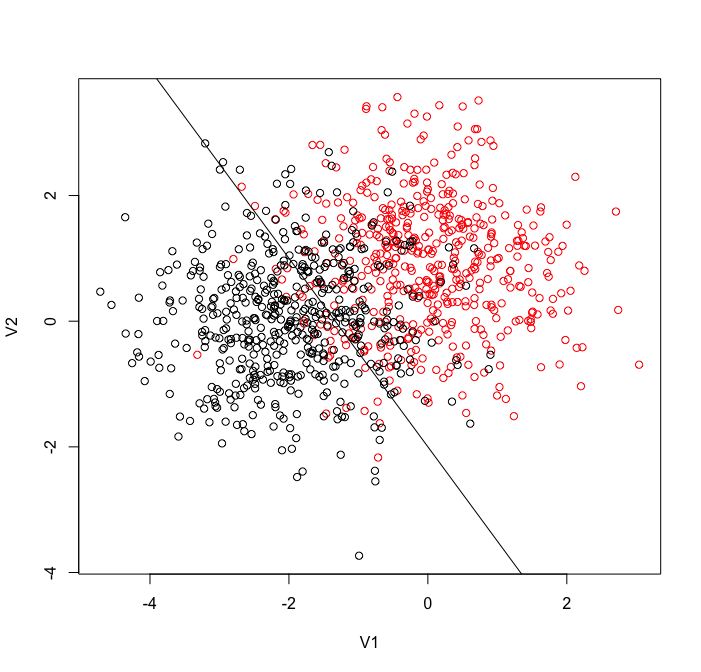
\includegraphics[width=.5\linewidth]{img/3-2-1-front-dec-euc-Synth1}
	\caption{\small Frontière de décision pour les données \textit{Synth-1000}}	
	\label{fig:3-2-1-front-dec-euc-Synth1}%
\end{figure}


\subsection{Règle de Bayes pour le jeu de données \textit{Synth2}}

On a ~:
\begin{align*}
\delta^*(x) = a_1 \quad 
&\Leftrightarrow \quad f_1(x) > f_2(x) \\
&\Leftrightarrow \quad -\frac{1}{2} (x - \mu_1)^t \Sigma_1^{-1} (x - \mu_1) - \frac{1}{2}\ln(|\Sigma_1|) > -\frac{1}{2} (x - \mu_2)^t \Sigma_2^{-1} (x - \mu_2)  -\frac{1}{2} \ln(|\Sigma_2|) \\
&\Leftrightarrow \quad - (x - \mu_1)^t \Sigma_1^{-1} (x - \mu_1) - \ln(|\Sigma_1|) > - (x - \mu_2)^t \Sigma_2^{-1} (x - \mu_2)  - \ln(|\Sigma_2|) \\
&\Leftrightarrow \quad (x - \mu_2)^t \Sigma_2^{-1} (x - \mu_2) - (x - \mu_1)^t \Sigma_1^{-1} (x - \mu_1) - \ln(|\Sigma_1|) + \ln(|\Sigma_2|) > 0 \\
\end{align*}

Or $\Sigma_{1} = diag(\sigma_{11}^2, \sigma_{12}^2)$ et $\Sigma_{2} = diag(\sigma_{21}^2, \sigma_{22}^2)$ (elles sont toutes deux diagonales)~:
\begin{align*}
\Sigma_{1}^{-1} &= \begin{pmatrix} 1/\sigma_{11}^2 & 0 \\ 0 & 1/\sigma_{12}^2 \end{pmatrix} \\
\Sigma_{2}^{-1} &= \begin{pmatrix} 1/\sigma_{21}^2 & 0 \\ 0 & 1/\sigma_{22}^2 \end{pmatrix} \\
|\Sigma_1| &= \sigma_{11}^2 . \sigma_{12}^2  \\
|\Sigma_2| &= \sigma_{21}^2 . \sigma_{22}^2  \\
\end{align*}


Calcul de $ (x - \mu_k)^t \Sigma_k^{-1} (x - \mu_k) $~:
\begin{align*}
(x - \mu_k)^t \Sigma_k^{-1} (x - \mu_k) 
&= ( x_1 - \mu_{k1}, x_2 - \mu_{k2}) \begin{pmatrix} \frac{1}{\sigma_{k1}^2} & 0 \\ 0 & \frac{1}{\sigma_{k2}^2} \end{pmatrix} \begin{pmatrix} x_1 - \mu_{k1} \\ x_2 - \mu_{k2} \end{pmatrix} \\
&=  \left( \frac{x_1 - \mu_{k1}}{\sigma_{k1}^2} , \frac{x_2 - \mu_{k2}}{\sigma_{k2}^2} \right) \begin{pmatrix} x_1 - \mu_{k1} \\ x_2 - \mu_{k2} \end{pmatrix} \\
&=   \frac{(x_1 - \mu_{k1})^2}{\sigma_{k1}^2} + \frac{(x_2 - \mu_{k2})^2}{\sigma_{k2}^2} \\
&= \frac{x_1^2 - 2x_1\mu_{k1} + \mu_{k1}^2}{\sigma_{k1}^2}
	+ \frac{x_2^2 - 2x_2\mu_{k2} + \mu_{k2}^2}{\sigma_{k2}^2} \\
&= \frac{x_1(x_1 - 2\mu_{k1})}{\sigma_{k1}^2}
	+ \frac{x_2(x_2 - 2\mu_{k2})}{\sigma_{k2}^2}
	+ \frac{\mu_{k1}^2}{\sigma_{k1}^2}
	+ \frac{\mu_{k2}^2}{\sigma_{k2}^2} \\
\end{align*}



On obtient donc~:
\begin{align*}
\delta^*(x) = a_1 \quad 
&\Leftrightarrow \quad f_1(x) > f_2(x) \\
&\Leftrightarrow \quad (x - \mu_2)^t \Sigma_2^{-1} (x - \mu_2) - (x - \mu_1)^t \Sigma_1^{-1} (x - \mu_1) - \ln(|\Sigma_1|) + \ln(|\Sigma_2|) > 0 \\
&\Leftrightarrow \quad 
	\frac{x_1(x_1 - 2\mu_{21})}{\sigma_{21}^2}
	+ \frac{x_2(x_2 - 2\mu_{22})}{\sigma_{22}^2}
	+ \frac{\mu_{21}^2}{\sigma_{21}^2}
	+ \frac{\mu_{22}^2}{\sigma_{22}^2} \\
&\qquad \qquad 
	- \frac{x_1(x_1 - 2\mu_{11})}{\sigma_{11}^2}
	- \frac{x_2(x_2 - 2\mu_{12})}{\sigma_{12}^2}
	- \frac{\mu_{11}^2}{\sigma_{11}^2}
	- \frac{\mu_{12}^2}{\sigma_{12}^2} \\
&\qquad \qquad - \ln(\sigma_{11}^2 \sigma_{12}^2) + \ln(\sigma_{21}^2 \sigma_{22}^2) > 0 \\
&\Leftrightarrow \quad 
	x_1 \left( 
		\frac{(x_1 - 2\mu_{21})}{\sigma_{21}^2} 
		- \frac{(x_1 - 2\mu_{11})}{\sigma_{11}^2}
	\right)
	+ x_2 \left( 
		\frac{(x_2 - 2\mu_{22})}{\sigma_{22}^2}
		- \frac{(x_2 - 2\mu_{12})}{\sigma_{12}^2}
	\right) \\
	&\qquad \qquad + \left(  
		\frac{\mu_{21}^2}{\sigma_{21}^2} 
		+ \frac{\mu_{22}^2}{\sigma_{22}^2} 
		+ \ln(\sigma_{21}^2 \sigma_{22}^2) 
	\right) \\
	&\qquad \qquad - \left(  
		\frac{\mu_{11}^2}{\sigma_{11}^2} 
		+ \frac{\mu_{12}^2}{\sigma_{12}^2} 
		+ \ln(\sigma_{11}^2 \sigma_{12}^2)
	\right) > 0
\end{align*}


La règle de Bayes $\delta^*(x)$ est donc fonction quadratique de $x = (x_1, x_2)^t$ et de deux constantes
\begin{align*}
c_1 &= - \left(  
\frac{\mu_{11}^2}{\sigma_{11}^2} 
+ \frac{\mu_{12}^2}{\sigma_{12}^2} 
+ \ln(\sigma_{11}^2 \sigma_{12}^2)
\right) \\
c_2 &= \left(  
\frac{\mu_{21}^2}{\sigma_{21}^2} 
+ \frac{\mu_{22}^2}{\sigma_{22}^2} 
+ \ln(\sigma_{21}^2 \sigma_{22}^2) 
\right)
\end{align*}


Si on remplace $\mu_{1}$, $\mu_{2}$, $\sigma_{1}^2$ et $\sigma_{2}^2$ par leurs valeurs numériques, on obtient~:
\begin{align*}
\delta^*(x) 
&=  \left\{ 
\begin{array}{l}
a_1 \quad si\ \frac{1}{5}(-4x_1^2 + 34x_1) + \left(c_1\right) + \left(c_2\right) > 0 \\
a_2 \quad sinon
\end{array} 	\right. \\
&=  \left\{ 
\begin{array}{l}
a_1 \quad si\ \frac{1}{5}(-4x_1^2 + 34x_1) + \frac{1}{5} \left( 4 - 45 + 5\ln(5) \right) > 0 \\
a_2 \quad sinon
\end{array} 	\right. \\
&=  \left\{ 
\begin{array}{l}
a_1 \quad si\ -4x_1^2 + 34x_1 > 41 - 5\ln(5) \\
a_2 \quad sinon
\end{array} 	\right.
\end{align*}


La frontière de décision a donc pour équation $-4x_1^2 + 34x_1 -41 + 5\ln(5) = 0$

\begin{figure}[H]
	\centering
	\captionsetup{justification=centering, margin=4cm}
	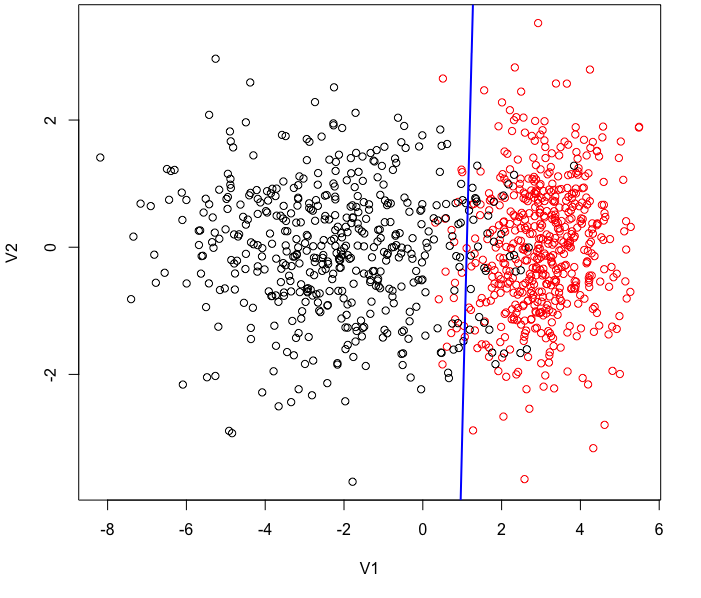
\includegraphics[width=.5\linewidth]{img/3-2-1-front-dec-euc-Synth2}
	\caption{\small Frontière de décision pour les données \textit{Synth-2000}}	
	\label{fig:3-2-1-front-dec-euc-Synth2}%
\end{figure}


\section{Calcul de l'erreur de Bayes}


\subsection{Jeu de données \textit{Synth1}}

Dans le cadre du classifieur euclidien, avec $\Sigma_k = \Sigma \ \forall \ k \in \{1, ...,  g\}$ diagonale et scalaire, $\pi_{1} = \pi_{2}$, l'erreur de Bayes est donnée par la formule suivante~:
\begin{align*}
	\epsilon^* = \phi \left(-\frac{\Delta}{2}\right)
\end{align*}
avec $\Delta^2 = (\mu_{2} - \mu_{1})^t\Sigma^{-1}(\mu_{2} - \mu_{1}) = 5$.\\


On obtient donc~:
\begin{align*}
\epsilon^* 
= \phi \left(-\frac{\Delta}{2}\right)
= \phi \left(-\frac{\sqrt{5}}{2}\right)
= 0.13
\end{align*}

On remarque que les estimation du taux d'erreur $ \hat{\epsilon}$ obtenues sur les données \textit{Synth1} (voir \autoref{subsection:estimation-erreur-synth1}) convergent vers la borne de l'erreur théorique $\epsilon^* = 0.13$ lorsque la taille des jeux de données augmente.

\subsection{Jeu de données \textit{Synth2}}

Dans le cadre des données \textit{Synth2}, on a toujours $\pi_{1} = \pi_{2}$, mais les matrices de variances ne sont plus égales entre-elles.\\

On va donc utiliser la borne de Bhattacharrya afin d'approximer l'erreur de Bayes~:
\begin{align*}
\epsilon^* &\leq \sqrt{\pi_{1}\pi_{2}} \int_{\mathbb{R}_p} \sqrt{f_1(x)f_2(x)}dx \\
\Leftrightarrow \quad \epsilon^* &\leq \sqrt{\pi_{1}\pi_{2}} \exp(-\Delta_B^2)
\end{align*}

Nous sommes dans le cas gaussien, alors~:
\begin{align*}
\Delta_B^2 = \frac{1}{8}(\mu_{2} - \mu_1)^t \left(\frac{\Sigma_{1} + \Sigma_{2}}{2}\right)^{-1} (\mu_{2} - \mu_1)
	+ \frac{1}{2} \ln \left( \frac{|\frac{\Sigma_{1} + \Sigma_{2}}{2}|}{\sqrt{|\Sigma_1||\Sigma_2|}} \right)
\end{align*}
peut être utilisée dans le calcul de la borne supérieure de l'erreur de Bayes.\\


On obtient finalement, après calcul, $\epsilon^* \leq 0.15$.

On remarque que les estimation du taux d'erreur $ \hat{\epsilon}$ obtenues sur les données \textit{Synth2} (voir \autoref{subsection:estimation-erreur-synth2}) est bien inférieure à la borne maximale de l'erreur de Bayes, car on avait obtenu $\hat{\epsilon}_{app} = 0.062$ et $\hat{\epsilon}_{test} = 0.063$.\\
Cela peut s'expliquer si l'on regarde l'estimation des paramètres, et plus particulièrement $\Sigma_{2}$~: la dispersion de la première variable $X^1$, sensée valoir $5$, vaut $4.43$ pour le jeu de données \textit{Synth2-1000}. On a une dispersion moins importante sur l'axe $X^1$ et donc une zone de chevauchement moins grande, d'où le faible taux d'erreur comparé à la borne maximale de l'erreur de Bayes.


























\appendix









\chapter{Fonction \texttt{compute.sucess.rate()}}
\label{annexe:compute.sucess.rate}
\begin{figure}[H]
	\centering
	\captionsetup{justification=centering, margin=4cm}
	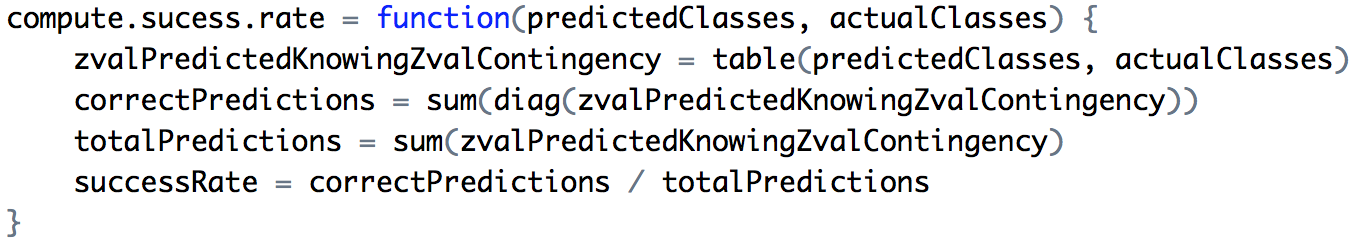
\includegraphics[width=.9\linewidth]{img/annexe-1-compute-sucess-rate}
	\caption{\small Code de la fonction \texttt{compute.sucess.rate()}}	
	\label{fig:annexe-1-compute-sucess-rate}%
\end{figure}



\end{document}